\chapter{Quark/hybrid stars}

\section{Introduction}

\TODO{Recapitulate main points of project thesis:}

In this chapter, we will study a hypothetical class of compact stars known as quark stars.
Let us summarize the main ingredients in this work.

\subsubsection{The Tolman-Oppenheimer-Volkoff equation}

We will find mass-radius solutions to the Tolman-Oppenheimer-Volkoff equation
\begin{subequations}
\begin{align}
	\odv{P}{r} &= -\frac{G m \epsilon(P)}{r^2 c^2} \left( 1 + \frac{P}{\epsilon(P)} \right) \left( 1 + \frac{4 \pi r^3 P}{m c^2} \right) \left( 1 - \frac{2 G m}{r c^2} \right)^{-1} , \\
	\odv{m}{r} &= \frac{4 \pi r^2 \epsilon(P)}{c^2} ,
\end{align}
\end{subequations}
that we derived in \cref{chap:tov}.
To do so, we integrate it from the center with $m(0) = 0$ and different central pressures $P(0) = P_c$ to the surface defined by $P(R) = 0$ and with corresponding mass $m(R) = M$.

\subsubsection{Equation of state from the grand canonical ensemble}

We will derive equations of state for quark matter by studying effective models of quantum chromodynamics in the zero-temperature approximation.
As we showed in \cref{chap:tft}, the partition function can be calculated as
\begin{equation}
	Z = \trace e^{-\beta (\hat{H} - \mu \hat{N})} = \oint \dif \phi e^{\int_0^\beta \dif \tau \int_V \dif^3 x \, \lagr_E } = e^{-\beta V \Omega} .
\end{equation}
Having found the partition function, we can calculate the
\begin{align}
	\Omega = -\frac{\log Z}{\beta V}, \\
	n = -\pdv{\Omega}{\mu}, \\
	P = -\Omega, \\
	\epsilon = -P + \mu n
\end{align}

\begin{itemize}
\item Tolman-Oppenheimer-Volkoff equation
\item Grand canonical ensemble / partition function: $Z = e^{-\beta V \Omega}$, $n = -\pdv{\Omega}/{\Omega}$, $P = -\Omega$, $\epsilon = -P + \mu n$
\item Charge neutrality and chemical equilibrium (new)
\item Stability/unstability of 2-flavor/3-flavor quark matter (new, for finding bag constant $B$, Bodmer-Witten conjecture)
\end{itemize}


Determine bag constant by:
two-flavor quark matter should be unstable,
three-flavor quark matter should be stable (Bodmer-Witten conjecture),
compared to iron-$56$ with $E/N_B = \epsilon/n_B = \SI{930}{\mega\electronvolt}$.
\begin{equation}
	\frac{\epsilon_3(0)}{n_B} < \SI{930}{\mega\electronvolt} < \frac{\epsilon_2(0)}{n_B} .
\label{eq:lsm:bag_stability}
\end{equation}

\TODO{titles}

\TODO{units, $\hbar = c = G = k_B = 1$ or not?}

\TODO{organize project and master thesis together}

\section{Electric charge neutrality and chemical equilibrium in stars}

\TODO{generally, see Halvor's detailed discussion about this}

When we solved the Tolman-Oppenheimer-Volkoff equations for ideal neutron stars in \cref{chap:nstars}, our lives were quite simple.
The stars consisted of only one charge neutral particle, and we simply eliminated its chemical potential to find the equation of state.
Now we will consider stellar models with a greater variety of particles and nonzero electric charge.

How do we now find the equation of state, when there is one chemical potential for each kind of particle?
The answer is to impose additional physical requirements of electric charge neutrality and chemical equilibrium.
With these conditions, we will relate all but one of the chemical potentials to each other, leaving only one independent variable that we will eliminate to find the equation of state.

\subsection{Global electric charge neutrality}

We can make a very simple classical argument for why there can be no \emph{global} net electric charge in stars by comparing Newton's law of gravity and Coulomb's law.
Consider a test particle of mass $m$ and electric charge $q$ on the surface $R$ from the center of a star with total mass $M$ and electric charge $Q$.
In an idealized situation, the test particle is affected by the gravitational and electrostatic force, so that the total outwards \TODO{radial?} force on it is
\begin{equation}
	F_\text{out} = -G \frac{M m}{R^2} + k_e \frac{Q q}{R^2} .
\end{equation}
Furthermore, suppose the star consists of $N$ particles weighing \TODO{weight $\rightarrow$ mass} no more than some heavy baryon with mass $m_B$, so $M < N M_B$ and $m < m_B$.
Any electrically charged particle has about one elementary charge $q \approx \pm e$.
If the star has an opposite charge $Q = \mp Z e$, then $F_\text{out} < 0$ and the test particle stays in the star.
On the other hand, if the star has a like charge $Q = \pm Z e$, then
\begin{equation}
	F_\text{out} > -G \frac{N m_B^2}{R^2} + k_e \frac{Z e^2}{R^2} .
\end{equation}
We then surely have $F_\text{out} > 0$, provided that the number of elementary charges per particle satisfies
\begin{equation}
	\frac{Z}{N} > \frac{G m_B^2}{k_e e^2} \approx 10^{-37} ,
\end{equation}
where we have assumed a typical baryon mass $m_B = m_p = \SI{1.67e-27}{\kilogram}$.
This corresponds to practically zero electric charge per particle in the star.

This means that particle are expelled from the star while $Z > 10^{-37} N$ until $Z$ has fallen to \emph{at least} $Z < 10^{-37} N$.
We conclude that for all practical purposes, stars are \emph{globally} electrically charge neutral.

\TODO{what about radius $r < R$ instead of $r=R$?}

\TODO{what about general relativity instead of Newtonian gravity?}

\TODO{what about contribution from pressure and other things to $F_\text{out}$?}

\TODO{can I recast inequality in charge per solar mass? see discussion at beginning of \url{www.if.ufrgs.br/hadrons/MMalheiro.pdf}}

\subsection{Local electric charge neutrality}

\TODO{non-understandable comment from Møte 4, Gibbs/Maxwell contstruction etc?}

\TODO{Glendenning has papers regarding local charge neutrality (?)}

The argument in the previous section shows that a star can have no \emph{total} electric charge, but it places absolutely no limitations on its \emph{distribution}.
Moreover, our approach to calculating equations of state is inherently \emph{local} -- we obtain the equation of state $\epsilon(P)$ by eliminating the density $n$ at any \emph{single point} from the energy density $\epsilon(n)$ and pressure $P(n)$.
To make use of electric charge neutrality in our approach, we will promote it from a \emph{global} constraint to a \emph{local} one.

\TODO{now explain...}

\TODO{TOV equation is derived by assuming ideal fluid in equilibrium -- would local charge destroy that?}

\TODO{draw inspiration from standard argument that $\vec{E} = 0$ everywhere inside a conductor?}

Satisfied by
\begin{equation}
	\sum_p q_p \, n(\mu_p) = 0 ,
\label{eq:lsm:charge_neutrality}
\end{equation}
where the sum is over all particles present, each with electric charge $q_p$.
In the zero-temperature approximation with the density \eqref{eq:nstars:density_zeroT}, this is satisfied if
\begin{equation}
	\sum_p q_p \left( \mu_p^2 - m_p^2 \right)^{3/2} = 0 .
\end{equation}

\subsection{Chemical equilibrium}

\TODO{introduce}

Important reactions
\begin{subequations}
\begin{align}
	d     &\leftrightarrow u + e + \bar{\nu}_e, \\
	s     &\leftrightarrow u + e + \bar{\nu}_e, \\
	s + u &\leftrightarrow u + d .
\end{align}
\end{subequations}
Assume neutrinos leave star \TODO{why?}.
Then chemical equilibrium implies
\begin{subequations}
\begin{align}
	\mu_d &= \mu_u + \mu_e, \\
	\mu_s &= \mu_u + \mu_e, \\
	\mu_s &= \mu_d .
\end{align}
\label{eq:lsm:chemical_equilibrium}
\end{subequations}
(the third follows automatically from the two first)

\section{Two-flavor quark-meson model}

\TODO{move this to the start?
The linear sigma model is an effective low-energy model of quantum chromodynamics, so accordingly we should take it seriously only in terms of the shifted fields around the stable ground states, and not in terms of the unshifted fields around the unstable equilibrium at the top of the Mexican hat.
}

\begin{figure}
\centering
\tikzsetnextfilename{potential}
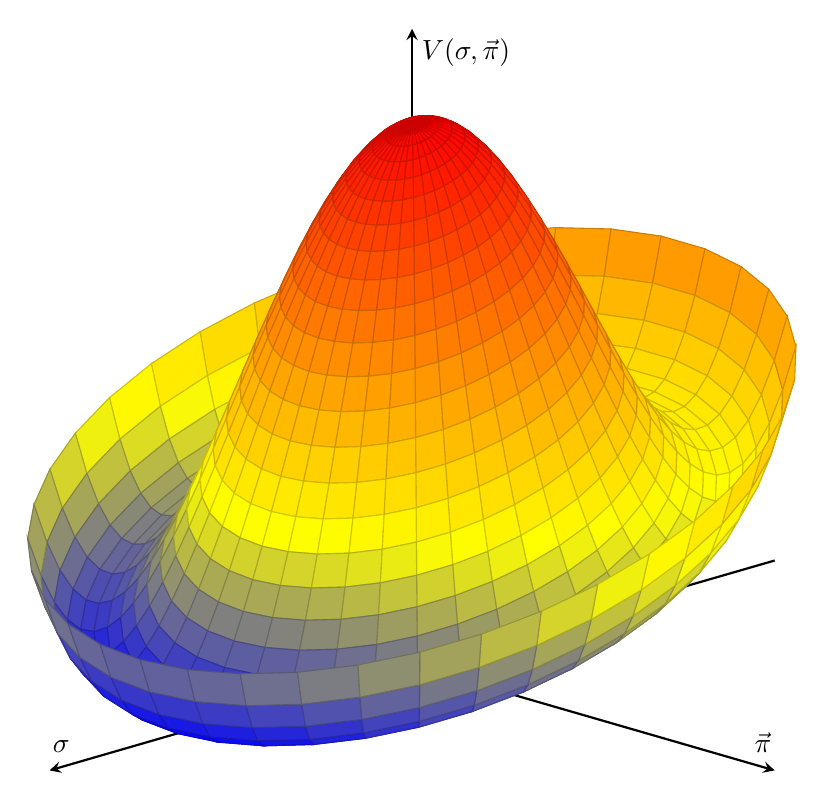
\begin{tikzpicture}
\begin{axis}[
	width = 20cm, height=15cm,
	%title = {Potential},
	xlabel = $\sigma$, ylabel = $\vec\pi$, zlabel = {$V(\sigma,\vec\pi)$},
	xmin=-4.0, xmax=+4.0, ymin=-4.0, ymax=+4.0, zmin=0, zmax=2.2,
	xtick=\empty, ytick=\empty, ztick=\empty,
	axis lines=center,
	axis line style = thick,
	view={135}{25},
	%colormap/blackwhite, mesh/interior colormap name=plasmarev,
]
	\addplot3 [surf, thin, domain=0:3.0, domain y=0:2*pi, samples=30, samples y=40, z buffer=sort] ({x*cos(deg(y))},{x*sin(deg(y))},{-1/2*((x*cos(deg(y)))^2+(x*sin(deg(y)))^2) + 1/24*((x*cos(deg(y)))^2+(x*sin(deg(y)))^2)^2 + 3/2 - 0.15*x*cos(deg(y)) + 0.15*sqrt(6)});
	%\addplot3 [domain=0:2*pi, samples=50, samples y=1] ({sqrt(6)*cos(deg(x))},{sqrt(6)*sin(deg(x))},{0});
\end{axis}
\end{tikzpicture}
\caption{\label{fig:lsm:potential}%
	A two-dimensional realization of the potential \eqref{eq:lsm:potential} looks like a Mexican hat, tilted along the $\sigma$-axis by the explicit symmetry breaking parameter $h$.
	If $h = 0$, the hat is upright with a continuous range of minima around $\sigma^2 + \vec\pi^2 = -6m^2 / \lambda$;
	while if $h \neq 0$, the hat is tilted and has the discrete minimum \eqref{eq:lsm:ground_state_implicit}.
}
\end{figure}

\TODO{justify this effective MODEL from QCD. Expand QCD $\lagr$ at low energy?}

The Lagrangian density for the linear sigma model coupled to quarks is
\begin{equation}
	\lagr = \sum_{c=1}^{N_c} \bar{q}_c \Big[ i \slashed\partial + \mu \gamma^0 - g \left( \sigma + i \gamma^5 \vec\tau \cdot \vec\pi \right) \Big] q_c
	      + \frac12 \left[ \left( \partial_\mu \sigma \right)^2 + \left( \partial_\mu \vec\pi \right)^2 \right] - \pot(\sigma,\vec\pi) ,
\label{eq:lsm:lagrangian}
\end{equation}
with the potential
\begin{equation}
	\pot(\sigma,\vec\pi) = \frac12 m^2 \left( \sigma^2 + \vec\pi^2 \right) + \frac{\lambda}{4!} \left( \sigma^2 + \vec\pi^2 \right)^2 - h \sigma .
	                     % = \frac{\lambda}{4!} \left( \sigma^2 + \vec\pi^2 - \frac{6m^2}{\lambda} \right)^2 -\frac{3 m^4}{2 \lambda} .
\label{eq:lsm:potential}
\end{equation}
This model is also called a quark-meson model.
Here $q_c = [u_c, d_c]^T$ represents quarks of the $N_c = 3$ colors red, green and blue and the $N_f = 2$ flavors up and down, so $(q_c)_f$ make up a total of $N_c \times N_f = 6$ Dirac spinors.
In addition, $\sigma$ and $\vec\pi = [\pi^+, \pi^-, \pi^0]^T$ are four bosonic scalar fields representing sigma and pion mesons.
At this point, the quarks are massless Dirac fermions whose conserved charge densities $j^0 = \bar\psi \gamma^0 \psi$ are coupled to chemical potentials $\mu = \diag(\mu_u, \mu_d)$, interacting with a Yukawa coupling of strength $g$ that models the strong force \TODO{non-mentioned comment in Møte 4}, where $\vec\tau$ are the Pauli matrices \eqref{eq:tft:pauli_matrices}.
\TODO{$SU(2)_L$, $SU(2)_R$, etc.?}

To make sense of this theory, we must investigate how it behaves around the classical ground state of the potential \eqref{eq:lsm:potential}.
If we imagine collapsing the three-dimensional $\vec{\pi}$ down to one dimension, the potential looks like the Mexican hat drawn in \cref{fig:lsm:potential}, tilted by the symmetry breaking parameter $h$.
Provided that $h \neq 0$, it has a discrete minimum located at
%Let us warm up with the special case $h = 0$, where the potential is symmetric under rotation of $[\sigma, \vec{\pi}]^T$ in $O(4)$ and looks like an upright Mexican hat with a continuous curve of minima along $\sigma^2 + \vec{\pi}^2 = -6m^2/\lambda$.
%Committing to one of these classical ground states, such as $\sigma=\avg{\sigma}=\sqrt{-6m^2/\lambda}$ and $\vec{\pi}=\avg{\vec{\pi}}=\vec{0}$,
%and shifting the fields to $\sigma \rightarrow \avg{\sigma} + \tilde{\sigma}$ and $\vec{\pi} \rightarrow \avg{\vec{\pi}} + \tilde{\vec{\pi}}$ then spontaneously breaks the symmetry to rotations of the pion quantum fluctuations $\tilde{\vec{\pi}}$ in $O(3)$ only,
%giving rise to three massless Goldstone bosons that we interpret as pions.
%We will work in the general case, however, where $h \neq 0$ tilts the hat so that it has a global minimum at $\sigma=\avg{\sigma}$ and $\vec{\pi}=\avg{\vec{\pi}}$ determined by
\begin{equation}
	\vec{\pi} = \avg{\vec{\pi}} = 0
	\quad \text{and} \quad
	\sigma = \avg{\sigma}
	\quad \text{where} \quad
	%\pdv{\pot}{\sigma}_{(\sigma,\vec\pi)=(\avg{\sigma},\vec{0})} = m^2 \avg{\sigma} + \frac{\lambda}{6} \avg{\sigma}^3 - h = 0.
	\pdv{\pot}{\sigma} = m^2 \avg{\sigma} + \frac{\lambda}{6} \avg{\sigma}^3 - h = 0.
\label{eq:lsm:ground_state_implicit}
\end{equation}
%We assume that $h \neq 0$, but will briefly discuss the qualitatively different behavior in the special case $h = 0$ in a moment.
To account for quantum fluctuations $\tilde{\sigma}$ and $\tilde{\vec{\pi}}$ around the classical ground state \eqref{eq:lsm:ground_state_implicit}, we shift
\begin{equation}
	\sigma \rightarrow \Avg{\sigma} + \tilde{\sigma}
	\qquad \text{and} \qquad
	\vec\pi \rightarrow \Avg{\vec\pi} + \tilde{\vec\pi}.
\label{eq:lsm:field_shift}
\end{equation}
In terms of the new fields $\tilde\sigma$ and $\tilde{\vec\pi}$, the Lagrangian \eqref{eq:lsm:lagrangian} is now
\begin{equation}
	\lagr = \sum_{c=1}^{N_c} \bar{q}_c \Big[ i \slashed\partial - m_q + \mu \gamma^0 - g \left( \tilde{\sigma} + i \gamma^5 \vec\tau \cdot \vec\pi \right) \Big] q_c
	      + \frac12 \left[ \left( \partial_\mu \tilde{\sigma} \right)^2 + \left( \partial_\mu \tilde{\vec\pi} \right)^2 \right] - \tilde{\pot}(\tilde{\sigma},\tilde{\vec\pi}) , %\pot(\avg{\sigma}+\tilde{\sigma},\avg{\vec\pi}+\tilde{\vec\pi}) ,
\end{equation}
where the quark fields $q$ have acquired field-dependent effective masses
\begin{equation}
	m_q(\avg{\sigma}) = g \avg{\sigma} .
\label{eq:lsm:mass_quark}
\end{equation}
The potential \eqref{eq:lsm:potential} up to second order in the shifted fields is
\begin{equation}
\begin{split}
	\tilde{\pot}(\tilde{\sigma},\tilde{\vec\pi}) &= \pot(\avg{\sigma}+\tilde{\sigma},\avg{\vec\pi}+\tilde{\vec\pi}) \\
	                                             &\taylor \frac12 m^2 \avg{\sigma}^2 + \frac{\lambda}{4!} \avg{\sigma}^4 - h \avg{\sigma} + \frac12 m_\sigma^2 \sigma^2  + \frac12 m_\pi^2 \vec\pi^2 ,
	%V(\sigma, \vec\pi) \taylor -\frac12 m^2 \avg{\sigma}^2 + \frac{\lambda}{4!} \avg{\sigma}^4 + \frac12 (\sqrt{2} m)^2 \sigma^2 .
	%V(\sigma, \vec\pi) \taylor -\frac{3 m^4}{2 \lambda} + \frac12 (\sqrt{2} m)^2 \sigma^2 .
\label{eq:lsm:potential_shifted}
\end{split}
\end{equation}
where the $\sigma$ and $\vec\pi$ fields have acquired the effective masses
\begin{subequations}
\begin{align}
	m_\sigma^2 &= \pdv[2]{\pot}{\sigma}_{(\sigma,\vec\pi)=(\avg{\sigma},\vec{0})}    = m^2 + \frac{\lambda}{2} \avg{\sigma}^2 \equalexplabove{\text{by \eqref{eq:lsm:ground_state_implicit}}} \frac{3h}{\avg{\sigma}} - 2 m^2 , \label{eq:lsm:mass_sigma} \\
	m_\pi^2    &= \pdv[2]{\pot}{\vec{\pi}}_{(\sigma,\vec\pi)=(\avg{\sigma},\vec{0})} = m^2 + \frac{\lambda}{6} \avg{\sigma}^2 \equalexplbelow{\text{by \eqref{eq:lsm:ground_state_implicit}}} \frac{h}{\avg{\sigma}} , \label{eq:lsm:mass_pi}
\end{align}%
\label{eq:lsm:mass_sigmapi}%
\end{subequations}%
The fate of the pion mass \eqref{eq:lsm:mass_pi} is determined by the presence of the symmetry breaking parameter $h$.
In the special case $h = 0$, the potential \eqref{eq:lsm:potential} shown in \cref{fig:lsm:potential} is rather shaped like an upright Mexican hat and is symmetric under rotations of $[\sigma,\vec{\pi}]^T$ in $O(4)$.
It then no longer has the \emph{discrete} minimum \eqref{eq:lsm:ground_state_implicit}, but a \emph{continuous} range of minima along the ``brim'' $\sigma^2 + \vec{\pi}^2 = -6m^2/\lambda$ of the hat.
Upon committing to one of these classical ground states, such as $\sigma=\avg{\sigma}=\sqrt{-6m^2/\lambda}$ and $\vec{\pi}=\avg{\vec{\pi}}=\vec{0}$ and performing the field shift \eqref{eq:lsm:field_shift},
the symmetry is \emph{spontaneously} broken down to rotations of only the pion quantum fluctuations $\tilde{\vec{\pi}}$ in $O(3)$.
This gives rise to three Goldstone bosons that we interpret as \emph{massless} pions, as confirmed by equation \eqref{eq:lsm:mass_pi} with $h = 0$.
We work in the general case, however, where $h \neq 0$ instead breaks the symmetry \emph{explicitly} by tilting the hat so it has the discrete minimum \eqref{eq:lsm:ground_state_implicit}, ultimately producing \emph{massive} pions, like those observed in nature.

We determine the four parameters $g$, $h$, $m$ and $\lambda$ in the original Lagrangian \eqref{eq:lsm:lagrangian} so that it yields the physical masses
\cite{ref:jo_lsm_renormalization}
\TODO{source?}
\begin{equation}
	m_q = \SI{300}{\mega\electronvolt}, \quad
	m_\pi = \SI{138}{\mega\electronvolt} \quad \text{and} \quad
	m_\sigma = \SI{800}{\mega\electronvolt} \quad \text{at} \quad
	\avg{\sigma} = f_\pi = \SI{93}{\mega\electronvolt}.
\end{equation}
Inverting equations \eqref{eq:lsm:ground_state_implicit}, \eqref{eq:lsm:mass_sigmapi} and \eqref{eq:lsm:mass_quark}, we then find the parameters
\begin{equation}
	g       = \frac{m_q}{f_\pi}, \quad % &\qquad& \text{(by \eqref{eq:lsm:mass_quark})} , \\
	h       = m_\pi^2 f_\pi, \quad % &\qquad& \text{(by \eqref{eq:lsm:mass_pi})} , \\
	m^2     = \frac{3m_\pi^2 - m_\sigma^2}{2} \quad \text{and} \quad % &\qquad& \text{(by \eqref{eq:lsm:mass_sigma})} , \\
	\lambda = \frac{3 m_\sigma^2 - 3 m_\pi^2}{f_\pi^2} .    % &\qquad& \text{(by \eqref{eq:lsm:ground_state_implicit})} .
\label{eq:lsm:parameters}
\end{equation}

According to what we learned in \cref{chap:tft} in \cref{eq:tft:boson_partition_function_momentum_out} and \eqref{eq:tft:dirac_partition_function_first},
the exact partition function corresponding to this theory is obtained by a path integral over periodic bosonic fields and anti-periodic fermionic fields, weighted by a Euclidean action in imaginary time:
\TODO{sign in exponent?}
\begin{equation}
	Z = \oint_- \pathintdif \bar{q} \oint_- \pathintdif q \oint_+ \pathintdif \sigma \oint_+ \pathintdif \vec\pi \exp \left\{ \int_0^\beta \dif \tau \int_V \dif^3 x \, \lagr_E[\bar{q}, q, \sigma, \vec\pi]  \right\} .
\end{equation}
As before, we are interested in $\log Z$ so we can calculate the thermodynamic quantities \eqref{eq:tft:average_quantities} and ultimately an equation of state $\epsilon(P)$, so we can solve the Tolman-Oppenheimer-Volkoff equation \eqref{eq:tov:tovsys}.
Here we will account for quantum effects of the quarks by treating them up to quadratic order (or one-loop),
but calculate only to zeroth order (or tree-level) in the meson fields and hence consider them only at the classical level.
The partition function then reads
\begin{equation}
\begin{split}
	Z &\taylor \oint_- \pathintdif \bar{q} \oint_- \pathintdif q \\
	  &\times  \exp \left\{ \int_0^{\beta} \dif \tau \int_V \dif^3 x \left[ \sum_{c=1}^{N_c} \bar{q}_c \left( i \slashed\partial -m_q + \mu \gamma^0 \right) q_c - \frac12 m^2 \avg{\sigma}^2 - \frac{\lambda}{4!} \avg{\sigma}^4 + h \avg{\sigma} \right] \right\} \\
	  &=       \prod_{f=1}^{\smash{N_f}} \prod_{c=1}^{\smash{N_c}} \oint_- \pathintdif \bar{q}_f^c \oint_- \pathintdif q_f^c \\
	  &\times  \exp \left\{ \int_0^{\beta} \dif \tau \int_V \dif^3 x \left[ \sum_{f=1}^{\smash{N_f}} \sum_{c=1}^{N_c} \bar{q}_f^c \left( i \slashed\partial - m_q + \mu_f \gamma^0 \right) q_f^c - \frac12 m^2 \avg{\sigma}^2 - \frac{\lambda}{4!} \avg{\sigma}^4 + h \avg{\sigma} \right] \right\}.
\end{split}
\end{equation}
The two last terms in the exponential are independent of the fields, so
\begin{equation}
\begin{split}
	\log Z &= -\frac12 \beta V m^2 \avg{\sigma}^2 - \frac{\lambda}{4!} \beta V \avg{\sigma}^4 + \beta V h \avg{\sigma} \\
	       &+ \sum_{f=1}^{N_f} \sum_{c=1}^{N_c} \log \oint_- \pathintdif \bar{q}_f^c \oint_- \pathintdif q_f^c \exp \left\{ \int_0^\beta \dif \tau \int_V \dif^3 x \, \bar{q}_f^c (i \slashed\partial + \mu_f \gamma^0 - m_q) q_f^c \right\} .
\end{split}
\end{equation}
We have already spent a great deal of effort in calculating the path integral in the last term,
starting from \cref{eq:tft:dirac_partition_function_first} and resulting in the expression \eqref{eq:tft:dirac_partition_function}.
Here, we get an additional factor $\sum_{c=1}^{N_c} = N_c$ from the color sum because the summand is independent of $c$,
while the flavor sum $\sum_{f=1}^{\smash{N_f}}$ yields $N_f$ terms that differ only by the unique chemical potentials $\mu_f$ associated with each quark flavor. 
Thus, we obtain
\begin{equation}
\begin{split}
	\log Z &= -\frac12 \beta V m^2 \avg{\sigma}^2 - \frac{\lambda}{4!} \beta V \avg{\sigma}^4 + \beta V h \avg{\sigma} \\
	       &+ 2 V N_c \sum_{f=1}^{N_f} \int \frac{\dif^3 p}{(2 \pi)^3} \left\{ \beta E(\vec{p}) + \log \left[ e^{-\beta (E(\vec{p}) - \mu_f)}+1 \right] + \log \left[ e^{-\beta (E(\vec{p}) + \mu_f)} + 1\right] \right\} ,
\end{split}
\label{eq:lsm:potential_divergent_logz0}
\end{equation}
where the dispersion relation is
\begin{equation}
	E(\vec{p}) = \sqrt{p^2 + m_q^2} .
\end{equation}
We can assess our approximation of treating bosons to tree-level, but fermions to loop-level from expression \eqref{eq:lsm:potential_divergent_logz0}.
The fermionic contribution in the second line is of order $\bigo(N_c^1)$, while the bosonic contribution in the first line is only of order $\bigo(N_c^0)$.
Thus, this approximation is exact in the so-called large-$N_c$ limit $N_c \gg 1$.
The million-dollar question that decides the accuracy of the approximation is then whether $N_c = 3 \gg 1$.
Although it may sound like we are not making a great case for ourselves, this is the most common treatment in the literature, and thus the strategy that we will adopt for now.
However, we will later return to this issue and consistently treat both bosons and fermions to the one-loop level, building upon the results of \cite{ref:jo_lsm_renormalization}.
\TODO{will I return to this later? RPA -- one-loop bosons too!}

Like in \cref{chap:nstars}, we assume that the chemical potentials are chosen so that anti-particles are more or less absent, so we drop their contribution in the last term in the second line.
From the middle term in the second line, we obtained the contribution $\log Z = \beta V P$ with the pressure \eqref{eq:nstars:pressure_zeroT} in the zero-temperature approximation, which we will continue to use.
This time, however, we will renormalize the infinite vacuum contribution from the first term in the second line, instead of simply dropping it, like we did back in \cref{chap:nstars}.
Thus, we obtain
\begin{equation}
\begin{split}
	\log Z &= -\frac12 \beta V m^2 \avg{\sigma}^2 - \frac{\lambda}{4!} \beta V \avg{\sigma}^4 + \beta V h \avg{\sigma} + N_c N_f \log Z_0 \\
	       &+ N_c \frac{m_q^4 \beta V}{24 \pi^2} \sum_{f=1}^{N_f} \left[ (2 x_f^3 - 3x_f) \sqrt{x_f^2 + 1} + 3 \asinh x_f \right],
\end{split}
\end{equation}
where $x_f = p_f / m_q$ are normalized Fermi momenta, $\mu_f = \smash{\sqrt{p_f^2 + m_q^2}}$ are Fermi energies and the vacuum contribution is
\begin{equation}
	\log Z_0 = 2 \beta V \int \frac{\dif^3 p}{(2 \pi)^3} \sqrt{p^2 + m_q^2 } .
\label{eq:lsm:vacuum_contribution_3dim}
\end{equation}
To renormalize the vacuum contribution, let us use dimensional regularization in the minimal subtraction scheme.
In $d = 3 - 2 \epsilon$ spatial dimensions, the vacuum contribution is
\begin{equation}
\begin{split}
	\log Z_0 &= 2 \beta V \Lambda^{3-d} \int \frac{\dif^d p}{(2 \pi)^d} \sqrt{p^2 + m_q^2} \\
	         &= 2 \beta V \Lambda^{3-d} \frac{2 \pi^{d/2}}{\Gamma(d/2)} \int_0^\infty \frac{\dif p \, p^{d-1}}{(2 \pi)^d} \sqrt{p^2 + m_q^2} .
\end{split}
\label{eq:lsm:vacuum_contribution_ddim}
\end{equation}
%\TODO{what happens to the dimensions of the potential $V$ (as consequence of requiring $\log Z$ to be dimensionless)? $V \rightarrow V \lambda^{-2\epsilon}$?}
We have also multiplied the integral by $\Lambda^{3-d}$,
where $\Lambda$ is some number with $\unit{\Lambda} = \unit{p}$,
so that $\unit{\lambda^{3-d} \dif^d p} = \unit{\dif^3 p}$ and $\log Z$ remains dimensionless in all dimensions.
There is nothing that forbids us from doing so, 
as the regulator still does its only job of reducing the new integral \eqref{eq:lsm:vacuum_contribution_ddim} to the old integral \eqref{eq:lsm:vacuum_contribution_3dim} when we send $\epsilon \rightarrow 0$,
only now in a way that is well-defined in all dimensions.
The momentum integral can be written as an analytical continuation of the \emph{Beta function} \cite{ref:beta_function}
\begin{equation}
	B(x,y) = \int_0^\infty \dif t \, \frac{t^{x-1}}{(1+t)^{x+y}} = \frac{\Gamma(x) \Gamma(y)}{\Gamma(x+y)}
\end{equation}
if we substitute $t = p^2/m_q^2$ with $\dif t = 2 p \dif p / m_q^2$.
We then find
\begin{equation}
\begin{split}
	\log Z_0 &= \beta V \Lambda^{3-d} m_q^{d+1} \frac{2 (4 \pi)^{-d/2}}{\Gamma\big(\frac{d}{2}\big)} \int_0^\infty \dif t \, \frac{t^{d/2-1}}{(1+t)^{-1/2}} \\
	         &= \beta V \Lambda^{3-d} m_q^{d+1} \frac{2 (4 \pi)^{-d/2}}{\Gamma\big(\frac{d}{2}\big)} \frac{\Gamma\big(\frac{d}{2}\big) \Gamma\big( \textstyle{-\frac{d+1}{2}} \big)}{\Gamma\big( \textstyle{-\frac{1}{2}} \big)} .
\end{split}
\end{equation}
We now cancel the two factors $\Gamma(d/2)$ and replace $\Gamma(-1/2) = -2\sqrt{\pi}$.
Then we insert $d = 3 - 2 \epsilon$ back and use the property $\Gamma(z) = \Gamma(z+1) / z$ twice to transport the argument of the Gamma function as close as possible to its pole at $0$,
where we use its asymptotic expansion $\Gamma(\epsilon) = 1/\epsilon + \gamma + \bigo(\epsilon)$ upon arrival.
Expanding everything to zeroth order in $\epsilon$ then yields
\begin{equation}
\begin{split}
	\log Z_0 &=       -\frac{\beta V m_q^4}{8 \pi^2} \left( 4 \pi \frac{\Lambda^2}{m_q^2} \right)^\epsilon \Gamma(-2 + \epsilon) \\
	         &\taylor -\frac{\beta V m_q^4}{16 \pi^2} \left( \frac{1}{\epsilon} + \log \frac{\Lambda^2}{m_q^2} + \frac32 - \gamma + \log 4 \pi \right) .
\end{split}
\label{eq:lsm:vacuum_contribution_final}
\end{equation}
In hindsight, we now see that we could get rid of the terms $-\gamma + \log 4 \pi$ if we had rather used the modified minimal subtraction scheme, where one rescales $\Lambda^2 \rightarrow \Lambda^2 e^\gamma / 4 \pi$.
With the vacuum contribution \eqref{eq:lsm:vacuum_contribution_final} in this renormalization scheme, the full logarithm \eqref{eq:lsm:potential_divergent_logz0} becomes
\begin{equation}
\begin{split}
	\log Z &= -\frac12 \beta V m^2 \avg{\sigma}^2 - \frac{\lambda}{4!} \beta V \avg{\sigma}^4 - N_c N_f \frac{\beta V m_q^4}{16 \pi^2} \left[ \frac{1}{\epsilon} + \frac{3}{2} + \log\left(\frac{{\Lambda}^2}{m_q^2}\right) \right] \\
	       &+ N_c \frac{m_q^4 \beta V}{24 \pi^2} \sum_{f=1}^{N_f} \left[ (2 x_f^3 - 3x_f) \sqrt{x_f^2 + 1} + 3 \asinh x_f \right] .
\end{split}
\end{equation}
This investigation has revealed that the term $-N_c N_f m_q^4 \beta V / 16 \pi^2 \epsilon$ is responsible for the divergence of the vacuum term.
We also see that the preceding term can shield us from the guilty criminal if we split the coupling 
\begin{equation}
	\lambda = \lambda_P + \delta\lambda
	\qquad \text{with the counterterm} \qquad
	\delta\lambda = -N_c N_f \frac{3 g^4}{2 \pi^2 \epsilon} .
\end{equation}
Accordingly, we determine $\lambda_P$ instead of $\lambda$ from equation \eqref{eq:lsm:parameters}.
\TODO{is this right?}
The finite and renormalized expression for $\log Z$ is now
\begin{equation}
\begin{split}
	\log Z &= -\frac12 \beta V m^2 \avg{\sigma}^2 - \frac{\lambda_P}{4!} \beta V \avg{\sigma}^4 + \beta V h \avg{\sigma} - N_c N_f \frac{\beta V m_q^4}{16 \pi^2} \left[ \frac{3}{2} + \log\left(\frac{{\Lambda}^2}{m_q^2}\right) \right] \\
	       &+ N_c \frac{m_q^4 \beta V}{24 \pi^2} \sum_{f=1}^{N_f} \left[ (2 x_f^3 - 3x_f) \sqrt{x_f^2 + 1} + 3 \asinh x_f \right] .
\end{split}
\end{equation}
From $\log Z$, we can finally build a bridge to thermodynamics with the grand potential density
\begin{equation}
\begin{split}
	\Omega = -\frac{\log Z}{\beta V} &= \frac12 m^2 \avg{\sigma}^2 + \frac{\lambda_P}{4!} \avg{\sigma}^4 - h \avg{\sigma} + N_c N_f \frac{m_q^4}{16 \pi^2} \left[ \frac{3}{2} + \log\left(\frac{{\Lambda}^2}{m_q^2}\right) \right] \\
	                                 &- N_c \frac{m_q^4}{24 \pi^2} \sum_{f=1}^{N_f} \left[ (2 x_f^3 - 3x_f) \sqrt{x_f^2 + 1} + 3 \asinh x_f \right] .
\end{split}
\end{equation}
The renormalization procedure has introduced an unknown parameter $\Lambda$.
To determine it, we require that the minimum of the grand potential \eqref{eq:lsm:grand_potential} remains at $\avg{\sigma} = f_\pi = \SI{93}{\mega\electronvolt}$ of the potential \eqref{eq:lsm:potential} when we are in vacuum.
The first three terms of the grand potential are precisely the potential \eqref{eq:lsm:potential}, and hence already minimal at $\avg{\sigma} = f_\pi$ by assumption.
In vacuum, all densities \eqref{eq:nstars:density_zeroT} and hence normalized Fermi momenta $x_f$ vanish, so the second line of the grand potential is also absent.
Then all it takes to meet our renormalization condition is that the only remaining term satisfies
\begin{equation}
	\pdv*{\left[ N_c N_f \frac{m_q^4}{16 \pi^2} \left( \frac32 + \log \frac{\Lambda^2}{m_q^2} \right) \right] }{\avg{\sigma}} = 0,
	\quad \text{yielding} \quad
	\Lambda = \frac{g f_\pi}{\sqrt{e}} = \SI{182}{\mega\electronvolt}.
\label{eq:lsm:potential_vacuum_minimum}
\end{equation}

To ensure the star is charge neutral, we spice our mixture of quarks and mesons with free electrons.
This amounts to adding one more fermion term to the Lagrangian
\begin{equation}
	\lagr \rightarrow \lagr + \bar{\psi}_e \big( i \slashed\partial + \mu_e \gamma^0 - m_e \big) \psi_e
	\qquad \text{with mass} \qquad
	m_e = \SI{0.5}{\mega\electronvolt}.
\end{equation}
Let us also reinstate the definition $x = p / m = \sqrt{\mu^2-m^2} / m$ that we made in equation \eqref{eq:nstars:everything_zeroT}, in order to make the dependence on $\mu$ and $\avg{\sigma}$ explicit.
With electrons, the grand potential \eqref{eq:lsm:grand_potential} becomes
\begin{equation}
\begin{split}
	\Omega(\avg{\sigma},\mu_u,\mu_d,\mu_e) &= \frac12 m^2 \avg{\sigma}^2 + \frac{\lambda_P}{4!} \avg{\sigma}^4 - h \avg{\sigma} + N_c N_f \frac{m_q^4}{16 \pi^2} \left[ \frac{3}{2} + \log\left(\frac{{\Lambda}^2}{m_q^2}\right) \right] \\
	                                       &- \frac{N_c}{24 \pi^2} \sum_{f=\{u,d\}} \left[ \left( 2 \mu_f^2 - 5 m_q^2 \right) \mu_f \sqrt{\mu_f^2 - m_q^2} + 3 m_q^4 \asinh \left( \sqrt{\frac{\mu_{\smash{f}}^2}{m_q^2}-1} \right) \right] \\
	                                       &- \frac{  1}{24 \pi^2} \left[ \left( 2 \mu_e^2 - 5 m_e^2 \right) \mu_e \sqrt{\mu_e^2 - m_e^2} + 3 m_e^4 \asinh \left( \sqrt{\frac{\mu_e^2}{m_e^2}-1} \right) \right] .
\end{split}
\label{eq:lsm:grand_potential}
\end{equation}
The particle densities corresponding to the grand potential \eqref{eq:lsm:grand_potential} are
\begin{subequations}
\begin{align}
	n_u &= -\pdv{\Omega}{\mu_u} = \frac{N_c}{3 \pi^2} \Big( \mu_u^2 - m_q^2 \Big)^{\frac32}, \\
	n_d &= -\pdv{\Omega}{\mu_d} = \frac{N_c}{3 \pi^2} \Big( \mu_d^2 - m_q^2 \Big)^{\frac32}, \\
	n_e &= -\pdv{\Omega}{\mu_e} = \frac{  1}{3 \pi^2} \Big( \mu_e^2 - m_e^2 \Big)^{\frac32}.
\end{align}%
\label{eq:lsm:particle_densities}%
\end{subequations}%
Remember that the effective quark mass $m_q = g \avg{\sigma}$ also depends on the field!
In addition, we implicitly take the real part of every square root $\sqrt{\mu^2 - m^2}$, or equivalently consider them as step functions $\Theta(\mu-m) \sqrt{\mu^2 - m^2}$.
The rigorous understanding of this can be traced back to the zero-temperature calculation of the pressure \eqref{eq:nstars:pressure_zeroT}, related to the grand potential density by $\Omega = -P$, in which the integrand contained a step function $\Theta(\mu-E(p)) = \Theta(\mu-\sqrt{m^2+p^2})$ and we took for granted that $\mu > m$.
In the opposite case $\mu < m$, the step function would cause the whole integral to vanish.

\begin{figure}
\centering
\tikzsetnextfilename{grand-potential-nonneutral}
\begin{tikzpicture}
\begin{groupplot}[
	group style={group size={1 by 2}, vertical sep=2.0cm},
	view={160}{30},
	width=0.9\textwidth, height=10cm,
	xlabel = {$\avg{\sigma} \, / \, \si{\mega\electronvolt}$}, ylabel = {$\mu \, / \, \si{\mega\electronvolt}$}, zlabel = {$\Omega(\avg{\sigma}, \mu) \, / \, (\SI{100}{\mega\electronvolt})^4$},
	colormap/OrRd, point meta min=0, point meta max=450,
	3d box=complete,
	unbounded coords=jump, % skip at nan (i.e. the phase transition)
	extra tick style={grid=major, grid style={dashed}},
	title style={text width={10cm}},
]
\nextgroupplot[
	zmin=-50, zmax=+200,
	xmin=-450, xmax=+450,
	xtick distance=100, %minor x tick num=5,
	ytick distance=100, %minor y tick num=3,
	title = {\subcaption{\label{fig:lsm:grand-potential-nonneutral-big}Large-scale form}},
];
\addplot3 [surf, very thin, mesh/ordering=x varies, point meta={abs(\thisrow{sigma})}] table [x=sigma, y=mu, z=omega] {../code/data/2flavpot_big.dat};
%\addplot3 [red]  table [x=sigma0, y=mu0, z=omega0] {../code/data/2flavpot.dat}; % plot line of minima
%\addplot  [gray] table [x=sigma0, y=mu0, z expr={-40}] {../code/data/2flavpot.dat}; % plot its "shadow" in bottom plane
\nextgroupplot[
	zmin=-40, zmax=+0,
	xmin=-149, xmax=+149,
	xtick distance=50, %minor x tick num=5,
	ytick distance=100, %minor y tick num=3,
	title = {\subcaption{\label{fig:lsm:grand-potential-nonneutral-small}Small-scale form}},
];
\addplot3 [surf, very thin, mesh/ordering=x varies, point meta={abs(\thisrow{sigma})}] table [x=sigma, y=mu, z=omega] {../code/data/2flavpot.dat};
\addplot3 [blue]  table [x=sigma0, y=mu0, z=omega0] {../code/data/2flavpot.dat}; % plot line of minima
\addplot  [gray] table [x=sigma0, y=mu0, z expr={-40}] {../code/data/2flavpot.dat}; % plot its "shadow" in bottom plane
\end{groupplot}
\end{tikzpicture}
\caption{\label{fig:lsm:grand-potential-nonneutral}%
	The grand potential \eqref{eq:lsm:grand_potential} with $\mu_e = 0$ and $\mu_u = \mu_d = \mu$.
	Upper panel \subref{fig:lsm:grand-potential-nonneutral-big} shows its asymptotic form as $\avg{\sigma} \rightarrow \pm \infty$, while lower panel \subref{fig:lsm:grand-potential-nonneutral-small} highlights the interesting region around $\SI{0}{\mega\electronvolt} \lesssim \avg{\sigma} \lesssim \SI{100}{\mega\electronvolt}$.
	The \textcolor{blue}{blue line} and its \textcolor{gray}{gray projection} corresponds to the fields $\avg{\sigma}(\mu)$ for which the potential has a minimum determined by $\pdv{\Omega}/{\avg{\sigma}} = 0$.
}
\end{figure}

We require that the mean field $\avg{\sigma}$ is a stable minimum of the grand potential,
so we determine it by solving
\TODO{introduce mean field as an ``order parameter''. why not parametrize with this?}
\begin{equation}
	\pdv{\Omega}{\avg{\sigma}} = 0.
\label{eq:lsm:potential_minimize}
\end{equation}

To get a feeling for the general shape of the grand potential \eqref{eq:lsm:grand_potential}, we visualize the special case with $\mu_e = 0$ and $\mu_u = \mu_d = \mu$ in \cref{fig:lsm:grand-potential-nonneutral}.
In this case, $\Omega(\avg{\sigma},\mu)$ is a function of only two variables, and the minimization condition \eqref{eq:lsm:potential_minimize} then leaves one free variable $\mu$ that parametrizes the other variable $\avg{\sigma}(\mu)$ and the grand potential $\Omega(\avg{\sigma}(\mu),\mu)$, as shown by the blue line in the figure.
From the figure, we see that:
\begin{itemize}
\item For $\mu < \SI{300}{\mega\electronvolt} = m_q(f_\pi)$, no square roots have real parts, so we are in vacuum with minimum at $\avg{\sigma} = f_\pi = \SI{93}{\mega\electronvolt}$, as we required in equation \eqref{eq:lsm:potential_vacuum_minimum}.
      The feature that a \emph{range} of chemical potentials characterizes the vacuum is called the \emph{Silver Blaze property}.
\item For $\SI{300}{\mega\electronvolt} < \mu \lesssim \SI{400}{\mega\electronvolt}$, the square roots have nonzero real parts and the minimum transitions quickly and continuously closer to zero, corresponding to a crossover.
      Despite its rapid change, the grand potential remains a smooth function, so this does \emph{not} correspond to a phase transition of any order.
\item For $\mu \gtrsim \SI{400}{\mega\electronvolt}$, the minimum approaches $\avg{\sigma} \rightarrow 0$ asymptotically, but never reaches it.
\end{itemize}
Our objective, however, is to determine the equation of state $\epsilon(P)$ in the general case where we take the conditions of charge neutrality \eqref{eq:lsm:charge_neutrality} and $\beta$-equilibrium \eqref{eq:lsm:chemical_equilibrium} into account, in addition to the condition of potential minimization \eqref{eq:lsm:potential_minimize}.
Using the densities \eqref{eq:lsm:particle_densities} and that up quarks, down quarks and electrons have respective charges $+(2/3)e$, $-(1/3)e$ and $-e$, we should now solve the \emph{system} of equations
\begin{subequations}
\begin{align}
	0 &= \pdv{\Omega}{\avg{\sigma}} , \label{eq:lsm:minsys_min} \\
	0 &= +\frac23 n_u - \frac13 n_d - n_e , \label{eq:lsm:minsys_charge} \\
	\mu_d &= \mu_u + \mu_e . \label{eq:lsm:minsys_equilibrium}
\end{align}%
\label{eq:lsm:minsys}%
\end{subequations}%
In this case $\Omega(\avg{\sigma},\mu_u,\mu_d,\mu_e)$ is a function of \emph{four} variables,
constrained by \emph{three} equations,
leaving \emph{one} free variable that parametrizes the others and thus the grand potential, pressure and energy density,
from which it can be eliminated to yield the equation of state.

\TODO{``variable'' or ``parameter''?. independent vs dependent variables.}

\TODO{rewrite}
Which variable should we use as the free variable?
In fact, some choices yield ill-defined parametrizations for which one value of the parameter corresponds to multiple values of another variable.
A well-defined parametrization should produce invertible functions.
For example, using $\mu_u$ as the free variable produces a well-defined parametrization of $\avg{\sigma}(\mu_u)$ when $m_\sigma \gtrsim \SI{900}{\mega\electronvolt}$, but an ill-defined one when $m_\sigma \lesssim \SI{900}{\mega\electronvolt}$.
Define quark chemical potential $\mu$ and isospin chemical potential $\mu_I$ by
\begin{equation}
	\mu_u = \mu + \mu_I
	\qquad \text{and} \qquad
	\mu_d = \mu - \mu_I .
\label{eq:lsm:quark_chemical_potential}
\end{equation}
By the chain rule, the quark chemical potential $\mu$ corresponds to the total quark density
\begin{equation}
	-\pdv{\Omega}{\mu} = -\pdv{\Omega}{\mu_u} \pdv{\mu_u}{\mu} - \pdv{\Omega}{\mu_d} \pdv{\mu_d}{\mu} = -\pdv{\Omega}{\mu_u} - \pdv{\Omega}{\mu_d} = n_u + n_d = n_q .
\end{equation}
Through trial and error, we have found that we get a well-defined parametrization by setting the free variable to the quark chemical potential
\TODO{$\mu_B$ and $n_B$}
\begin{equation}
	\mu = \frac12 (\mu_u + \mu_d) .
\end{equation}

\begin{figure}
\centering
\tikzsetnextfilename{2-flavor-eos}
\begin{tikzpicture}
\begin{groupplot}[
	group style={group size={1 by 3}, vertical sep=2.0cm},
	width=13cm, height=7cm,
	extra tick style={grid=major, grid style={dashed}},
	minor tick num=9,
]
\nextgroupplot[
	xlabel={$\mu \, / \, \si{\mega\electronvolt}$},
	xmin=0, xmax=600, ymax=500, xtick distance=100, ytick distance=100, minor x tick num=9,
	%ymax=600, 
	title={\subcaption{\label{fig:lsm:2-flavor-eos-parametrization}Parametrization of solutions}},
	legend cell align=right, legend pos=north west,
];
\addplot+ [orange!50!white, densely dashed, semithick, opacity=0.7, forget plot] table [x=mu, y expr=0] {../code/data/2flavfreeeos.dat}; %\addlegendentry{$\avg{\sigma} \, / \, \si{\mega\electronvolt}$};
\addplot+ [orange, solid, opacity=0.7] table [x=mu, y=sigma] {../code/data/2flaveos.dat}; \addlegendentry{$\avg{\sigma} \, / \, \si{\mega\electronvolt}$};
\addplot+ [red!50!white, densely dashed, semithick, opacity=0.7, forget plot] table [x=mu, y=muu   ] {../code/data/2flavfreeeos.dat}; %\addlegendentry{$\mu_u \, / \, \si{\mega\electronvolt}$};
\addplot+ [red, solid, opacity=0.7] table [x=mu, y=muu] {../code/data/2flaveos.dat}; \addlegendentry{$\mu_u \, / \, \si{\mega\electronvolt}$};
\addplot+ [darkgreen!50!white, densely dashed, semithick, opacity=0.7, forget plot] table [x=mu, y=mud   ] {../code/data/2flavfreeeos.dat}; %\addlegendentry{$\mu_d \, / \, \si{\mega\electronvolt}$};
\addplot+ [darkgreen, solid, opacity=0.7] table [x=mu, y=mud] {../code/data/2flaveos.dat}; \addlegendentry{$\mu_d \, / \, \si{\mega\electronvolt}$};
\addplot+ [blue!50!white, densely dashed, semithick, opacity=0.7, forget plot] table [x=mu, y=mue   ] {../code/data/2flavfreeeos.dat}; %\addlegendentry{$\mu_e \, / \, \si{\mega\electronvolt}$};
\addplot+ [blue, solid, opacity=0.7] table [x=mu, y=mue] {../code/data/2flaveos.dat}; \addlegendentry{$\mu_e \, / \, \si{\mega\electronvolt}$};


\nextgroupplot[
	xlabel={$\mu \, / \, \si{\mega\electronvolt}$}, ylabel={$n_i \, / \, (1/\si{\femto\meter\cubed})$},
	xmin=0, xmax=600, xtick distance=100, minor x tick num=9,
	ymax=2.0, ytick distance=0.5, minor y tick num=4,
	title={\subcaption{\label{fig:lsm:2-flavor-eos-density}Particle number densities}},
	legend cell align=left, legend pos=north west,
];
\coordinate (zoomplot) at (232, 1.32);
\draw [draw=none, fill=gray!50] (250, -0.005) rectangle (350, 0.02);
\draw [-Latex, gray] (300,0.03) to [out=90, in=0] (232, 0.75);
\addplot+ [red, densely dashed, semithick, opacity=0.7, forget plot] table [x=mu, y=nu] {../code/data/2flavfreeeos.dat};
\addplot+ [red, solid, opacity=0.7] table [x=mu, y=nu] {../code/data/2flaveos.dat}; \addlegendentry{$n_u$ (up quarks)};
\addplot+ [darkgreen, densely dashed, semithick, opacity=0.7, forget plot] table [x=mu, y=nd] {../code/data/2flavfreeeos.dat};
\addplot+ [darkgreen, solid, opacity=0.7] table [x=mu, y=nd] {../code/data/2flaveos.dat}; \addlegendentry{$n_d$ (down quarks)};
\addplot+ [blue, densely dashed, semithick, opacity=0.7, forget plot] table [x=mu, y=ne] {../code/data/2flavfreeeos.dat};
\addplot+ [blue, solid, opacity=0.7] table [x=mu, y=ne] {../code/data/2flaveos.dat}; \addlegendentry{$n_e$ (electrons)};

\nextgroupplot[
	xlabel={$P        \, / \, (\si{\giga\electronvolt\per\femto\meter\cubed})$},
	ylabel={$\epsilon \, / \, (\si{\giga\electronvolt\per\femto\meter\cubed})$},
	xmin=0, xmax=0.5, ymin=0, ymax=2, xtick distance=0.1, ytick distance=0.5, minor y tick num=4,
	title={\subcaption{\label{fig:lsm:2-flavor-eos-eos}Equation of state}},
	legend cell align=left, legend pos=north west,
];
\addplot+ [black, densely dashed, semithick, opacity=0.7, forget plot] table [x=P,y=epsilon] {../code/data/2flavfreeeos.dat}; %\addlegendentry{without interactions};
\addplot+ [black, solid, opacity=0.7] table [x=P,y=epsilon] {../code/data/2flaveos.dat};
\end{groupplot}
% Embed zoom-plot in a node
\node [anchor=north east] at (zoomplot) {
	\begin{tikzpicture}[baseline, trim axis left, trim axis right]
	\begin{axis}[
		width=4cm, height=3.5cm,
		scaled ticks=false,
		xmin=250, xmax=350, xtick distance=50, minor x tick num=4, yticklabel style={/pgf/number format/fixed, /pgf/number format/precision=3},
		ymin=-0.005, ymax=0.02, ytick distance=0.01, minor y tick num=9, restrict y to domain=-0.5:0.5,
		axis background/.style={fill=gray!50},
	]
	\addplot+ [red, densely dashed, semithick, opacity=0.7, forget plot] table [x=mu, y=nu] {../code/data/2flavfreeeos.dat};
	\addplot+ [red, solid, opacity=0.7] table [x=mu, y=nu] {../code/data/2flaveos.dat};
	\addplot+ [darkgreen, densely dashed, semithick, opacity=0.7, forget plot] table [x=mu, y=nd] {../code/data/2flavfreeeos.dat};
	\addplot+ [darkgreen, solid, opacity=0.7] table [x=mu, y=nd] {../code/data/2flaveos.dat};
	\addplot+ [blue, densely dashed, semithick, opacity=0.7, forget plot] table [x=mu, y=ne] {../code/data/2flavfreeeos.dat};
	\addplot+ [blue, solid, opacity=0.7] table [x=mu, y=ne] {../code/data/2flaveos.dat};
	\end{axis}
	\end{tikzpicture}
};
\end{tikzpicture}
\caption{\label{fig:lsm:2-flavor-eos}%
Properties of electrically charge neutral two-flavor quark matter in $\beta$-equilibrium parametrized by the quark chemical potential $\mu = (\mu_u+\mu_d)/2$.
Solid lines show
\subref{fig:lsm:2-flavor-eos-parametrization} solutions to the system of equations \eqref{eq:lsm:minsys} and the corresponding
\subref{fig:lsm:2-flavor-eos-density} particle number densities \eqref{eq:lsm:particle_densities} and
\subref{fig:lsm:2-flavor-eos-eos} equation of state \eqref{eq:lsm:eos}.
In comparison, dashed lines show the approximate analytical solutions \eqref{eq:lsm:chemical_potentials_massless}, \eqref{eq:lsm:densities_massless} and \eqref{eq:lsm:eos_massless} for a free quark gas in the massless limit $\avg{\sigma} = 0$ and $m_e = 0$.
}
\end{figure}

The numerical solution of the system \eqref{eq:lsm:minsys} is described in \cref{sec:num:qstars2f}, and the results are shown in \cref{fig:lsm:2-flavor-eos}.
\Cref{fig:lsm:2-flavor-eos-parametrization} shows the parametrization of the four arguments $\avg{\sigma}(\mu)$, $\mu_u(\mu)$, $\mu_d(\mu)$ and $\mu_e(\mu)$.
From these parametrizations, we compute the particle number densities \eqref{eq:lsm:particle_densities} in \cref{fig:lsm:2-flavor-eos-density}.
Finally, from the parametrizations and densities, we compute the pressure
\begin{subequations}
\begin{equation}
	P(\mu) = -\Big[\Omega(\mu) - \Omega(\mu<\SI{300}{\mega\electronvolt})\Big]
\label{eq:lsm:pressure_bagless}
\end{equation}
relative to vacuum and the energy density
\begin{equation}
	\epsilon(\mu) = -P(\mu) + \sum_i \mu_i(\mu) \, n_i(\mu) ,
\label{eq:lsm:energy_density_bagless}
\end{equation}%
\label{eq:lsm:eos}%
\end{subequations}%
then at last eliminate the free parameter $\mu$ to find the equation of state $\epsilon(P)$ in \cref{fig:lsm:2-flavor-eos-eos}.

As $\mu$ increases, the numerical results in \cref{fig:lsm:2-flavor-eos-parametrization} indicate that $\avg{\sigma}$ decays towards zero.
Let us leverage this to validate our numerical results to the analytical solution of the massless and non-interacting problem with $\avg{\sigma} = 0$,
where the quark mass $m_q = g \avg{\sigma} = 0$ and all other interaction terms vanish.
For simplicity, we also neglect the electron mass $m_e = 0$, as it is very light.
We expect correspondence with our numerical results for large values of $\mu$.
In this limit, the grand potential \eqref{eq:lsm:grand_potential} reduces to
\begin{equation}
	\Omega(\mu_u, \mu_d, \mu_e) = -\frac{N_c \mu_u^4}{12 \pi^2} - \frac{N_c \mu_d^4}{12 \pi^2} - \frac{\mu_e^4}{12 \pi^2},
\label{eq:lsm:grand_potential_massless}
\end{equation}
while the densities \eqref{eq:lsm:particle_densities} become
\begin{equation}
	n_u = \frac{N_c \abs{\mu_u}^3}{3 \pi^2}, \qquad
	n_d = \frac{N_c \abs{\mu_d}^3}{3 \pi^2}  \qquad \text{and} \qquad
	n_e = \frac{N_c \abs{\mu_e}^3}{3 \pi^2}.
\label{eq:lsm:densities_massless}
\end{equation}
The charge neutrality condition \eqref{eq:lsm:minsys_charge} can be solved approximately under the assumption that we can neglect the electron density $n_e \ll n_u < n_d$,
motivated by the faint electron density in the numerical solution.
This simplifies the condition to $n_d = 2 n_u$, with the solution $\mu_d = 2^{1/3} \mu_u$.
According to the $\beta$-equilibrium condition \eqref{eq:lsm:minsys_equilibrium},
the chemical potential of the electrons is $\mu_e = \mu_d - \mu_u = (1-2^{1/3}) \mu_u$,
corresponding to the density $n_e = (2^{1/3}-1)^3 n_u / N_c = 0.006 \, n_u \ll n_u$,
which is indeed negligible in line with our original assumption.
Summarizing and expressing these chemical potentials in terms of the quark chemical potential $\mu = (\mu_u+\mu_d)/2$ we have
\begin{equation}
	\mu_u = \frac{2}{1+2^{1/3}} \mu, \qquad
	\mu_d = \frac{2}{1+2^{-1/3}} \mu \qquad \text{and} \qquad
	\mu_e = (2^{1/3}-1) \mu.
\label{eq:lsm:chemical_potentials_massless}
\end{equation}
Using the grand potential \eqref{eq:lsm:grand_potential_massless} and densities \eqref{eq:lsm:densities_massless} ignoring the normalization of the pressure $P = -\Omega$, the equation of state is now
\begin{equation}
	\epsilon = -P + \sum_i \mu_i n_i = -P + \frac{1}{3 \pi^2} \Big(N_c \mu_u^4 + N_c \mu_d^4 + \mu_e^4\Big) = -P - 4 \Omega = -P + 4 P = 3 P .
\end{equation}
This is the same ultra-relativistic equation of state that we also found in equation \eqref{eq:nstars:ur_eos}.
To compare it with our numerical equation of state, we should normalize the pressure $P \rightarrow P + \Omega(\mu<\SI{300}{\mega\electronvolt})$ using the vacuum value of the grand potential that we obtained in our general analysis.
Doing so, we end up with the equation of state
\begin{equation}
	\epsilon = 3 P + 3 \Omega(\mu<\SI{300}{\mega\electronvolt}).
\label{eq:lsm:eos_massless}
\end{equation}
The analytical results \eqref{eq:lsm:chemical_potentials_massless}, \eqref{eq:lsm:densities_massless} and \eqref{eq:lsm:eos_massless} are also shown for comparison in \cref{fig:lsm:2-flavor-eos}, and agree with our numerical results for large $\mu$, as we expected.

A discussion of the results in \cref{fig:lsm:2-flavor-eos} is now in order:
\begin{itemize}
\item For $\mu < \SI{300}{\mega\electronvolt} = m_q(f_\pi)$, no square roots in the grand potential \eqref{eq:lsm:grand_potential} nor the densities \eqref{eq:lsm:particle_densities} have real parts, so we are in vacuum with the trivial solutions $\avg{\sigma} = f_\pi = \SI{93}{\mega\electronvolt}$, $\mu_e = 0$ and $\mu_u = \mu_d = \mu$ of equation \eqref{eq:lsm:minsys}, showing the Silver Blaze property again.
\item For $\SI{300}{\mega\electronvolt} < \mu \lesssim \SI{400}{\mega\electronvolt}$, the square roots acquire real parts and the system exhibits a crossover where particle densities increase rapidly from their vanishing vacuum values, while $\avg{\sigma}$ and hence the effective quark mass $m_q = g \avg{\sigma}$ plummets towards zero.
\item For $\mu \gtrsim \SI{400}{\mega\electronvolt}$, the potential minimum approaches $\avg{\sigma} \rightarrow 0$ asymptotically.
      Due to the small quark masses $m_q = g \avg{\sigma} \rightarrow 0$, the results in this region agree with the free quark gas results \eqref{eq:lsm:densities_massless}, \eqref{eq:lsm:chemical_potentials_massless} and \eqref{eq:lsm:eos_massless} in the massless limit.
\item Although the electrons have an appreciable chemical potential $\mu_e$, the electron \emph{density} $n_e$ is hardly noticeable compared to the quark densities $n_u$ and $n_d$.
      The magnified plot in \cref{fig:lsm:2-flavor-eos-density} shows that the electron density is \emph{nonzero}, only several orders of magnitude below the quark densities.
      This is consistent with the densities corresponding to the chemical potentials \eqref{eq:lsm:chemical_potentials_massless} that we found in the massless limit by neglecting the electron contribution to the charge neutrality condition \eqref{eq:lsm:minsys_charge}.
\item When normalized to the exact same vacuum pressure, the massive and massless equations of state in \cref{fig:lsm:2-flavor-eos-eos} agree for $P \rightarrow \infty$, which corresponds to $\mu \rightarrow \infty$ and in turn $\avg{\sigma} \rightarrow 0$ and $m_q = g \avg{\sigma} \rightarrow 0$, and hence massless quarks.
      For small pressures, however, the assumption of massless quarks breaks down and the two disagree.
\item \TODO{$m_\sigma$ value, two solutions to charge neutrality?}
\end{itemize}
We see that the crossover behavior is very similar to that in \cref{fig:lsm:grand-potential-nonneutral}.

\TODO{needs a small intro and rewriting...}
In addition, we will allow for a bag constant $B$ to be added to the pressure and energy density
\TODO{understand bag-constant as a measure of the trace anomaly? $m = 0$ -- conformal inveriance, classical symmetry broken in the quantum case?}
\TODO{justify and make less ad-hoc, move some of this to intro?}
\TODO{understand difference between $P(\mu)$ and $P(\mu,B)$}
\TODO{find source on bag stuff. JO?}
\TODO{difference between ``perturbative vacuum'' and ``confined vacuum''}
\begin{equation}
	P(\mu,B) = P(\mu) - B
	\qquad \text{and} \qquad
	\epsilon(\mu,B) = \epsilon(\mu) + B.
\end{equation}
The equation of state then depends on the value we choose for the bag constant.
To determine acceptable values for it, we use that two-flavor quark matter is not observed in nature, and so should be unstable with respect to the most stable form of baryonic matter, $^{56}\text{Fe}$, with an energy of $E/N_B = \SI{930}{\mega\electronvolt}$ per baryon.
We therefore choose $B$ so that the energy per baryon of two-flavor quark matter satisfies
\begin{subequations}
\begin{equation}
	\frac{E_2}{N_B} = \frac{\epsilon_2}{n_B} > \SI{930}{\mega\electronvolt} \quad \text{at} \quad P(\mu,B)=0,
\label{eq:lsm:bag_stability_2f}
\end{equation}
where $\epsilon_2 = \sum_i \mu_i n_i$ is the energy density of baryons at zero pressure, and the baryon number density is $n_B = N_B/V = (n_u + n_d)/3$.
Solving equation \eqref{eq:lsm:bag_stability_2f} numerically in \cref{sec:num:qstars2f} then yields the lower bag constant bound
\begin{equation}
	B > (\SI{27.2}{\mega\electronvolt})^4.
\label{eq:lsm:bag_lower_bound}
\end{equation}
\end{subequations}

\begin{figure}[t]
\centering
\tikzsetnextfilename{2-flavor-mass-radius}
\begin{tikzpicture}
\begin{axis}[
	width=15cm, height=12cm,
	xlabel={$R \, / \, \si{\kilo\meter}$}, ylabel={$M \, / \, M_\odot$}, title={Mass-radius diagram for 2-flavor quark stars}, title style={yshift=2.0cm},
	xmin=7, xmax=18, ymin=0.5, ymax=2, xtick distance=1, ytick distance=0.1, minor tick num=9, grid=major,
	point meta=explicit, point meta min=32, point meta max=39,
	colorbar horizontal, colormap name=plasmarev, colorbar style={xlabel=$\log_{10} (P_c \, / \, \si{\pascal})$, xtick distance=1, minor x tick num=9, at={(0.5,1.03)}, anchor=south, xticklabel pos=upper},
	declare function={
		e0 = 4.266500881855304e+37;
	},
	legend pos=north east, legend cell align=right,
]
\tikzset{
	Bpin/.style={gray, sloped, allow upside down=true, rotate=180, yshift=+0.4cm, font=\small},
}
\addplot+ [black, solid] {0};
\addlegendentry{stable stars};
\addplot+ [black, densely dashed] {0};
\addlegendentry{unstable stars};

\addplot+ [solid,          mesh, x filter/.expression={\thisrow{P} < 0.00139 ? x : nan}] table [x=R, y=M, meta expr={log10(\thisrow{P}*e0)}] {../code/data/quarkstar2f_B14_27.dat} node [Bpin, pos=0.82] {$B = (\SI{27}{\mega\electronvolt})^4$};
\addplot+ [densely dashed, mesh, x filter/.expression={\thisrow{P} > 0.00138 ? x : nan}] table [x=R, y=M, meta expr={log10(\thisrow{P}*e0)}] {../code/data/quarkstar2f_B14_27.dat};

\addplot+ [solid,          mesh, x filter/.expression={\thisrow{P} < 0.0015 ? x : nan}] table [x=R, y=M, meta expr={log10(\thisrow{P}*e0)}] {../code/data/quarkstar2f_B14_34.dat} node [Bpin, pos=0.77] {$B = (\SI{34}{\mega\electronvolt})^4$};
\addplot+ [densely dashed, mesh, x filter/.expression={\thisrow{P} > 0.0014 ? x : nan}] table [x=R, y=M, meta expr={log10(\thisrow{P}*e0)}] {../code/data/quarkstar2f_B14_34.dat};

\addplot+ [solid,          mesh, x filter/.expression={\thisrow{P} < 0.0013 ? x : nan}] table [x=R, y=M, meta expr={log10(\thisrow{P}*e0)}] {../code/data/quarkstar2f_B14_41.dat} node [Bpin, pos=0.70] {$B = (\SI{41}{\mega\electronvolt})^4$};
\addplot+ [densely dashed, mesh, x filter/.expression={\thisrow{P} > 0.0012 ? x : nan}] table [x=R, y=M, meta expr={log10(\thisrow{P}*e0)}] {../code/data/quarkstar2f_B14_41.dat};

\addplot+ [solid,          mesh, x filter/.expression={\thisrow{P} < 0.0016 ? x : nan}] table [x=R, y=M, meta expr={log10(\thisrow{P}*e0)}] {../code/data/quarkstar2f_B14_48.dat} node [Bpin, pos=0.47] {$B = (\SI{48}{\mega\electronvolt})^4$};
\addplot+ [densely dashed, mesh, x filter/.expression={\thisrow{P} > 0.0015 ? x : nan}] table [x=R, y=M, meta expr={log10(\thisrow{P}*e0)}] {../code/data/quarkstar2f_B14_48.dat};

\end{axis}
\end{tikzpicture}
\caption{\label{fig:lsm:2-flavor-mass-radius}Mass-radius solutions of the Tolman-Oppenheimer-Volkoff equations \eqref{eq:tov:tovsys} parametrized by central pressure $P_c$, obtained with the equation of state for two-flavor quark matter in \cref{fig:lsm:2-flavor-eos-eos} modified by a range of bag constants above the bound \eqref{eq:lsm:bag_lower_bound}.}
\end{figure}

With the equation of state, we now solve the Tolman-Oppenheimer-Volkoff equations \eqref{eq:tov:tovsys} with multiple bag pressures above the lower bound \eqref{eq:lsm:bag_lower_bound}.
This yields the central pressure-parametrized mass-radius curves in \cref{fig:lsm:2-flavor-mass-radius}, producing maximum masses up to $M < 1.77 M_\odot$.

\TODO{explain the solutions in the plots, and plot densities logarithmically?}

\TODO{just drop this part?
Having described we \emph{do} and \emph{should do}, let us also remark on what we \emph{did} and \emph{shouldn't do}.
A tempting and similar approach to minimizing $\Omega$ with respect to $\avg{\sigma}$ is to rather construct the potential $\Omega'(\avg{\sigma}, \mu_u) = \Omega(\avg{\sigma}, \mu_u, \mu_d(\mu_u,\avg{\sigma}), \mu_e(\mu_u,\avg{\sigma}))$, then minimize $\Omega'$ with respect to $\avg{\sigma}$.
In this approach, we could create two functions $\mu_{d/e}(\avg{\sigma},\mu_u)$ that calculate the two remaining chemical potentials by solving the charge neutrality condition \eqref{eq:lsm:minsys_charge} with a simple scalar root finder, both of which would be invoked upon evaluating the new potential $\Omega'(\avg{\sigma},\mu_u)$.
This sounds really nice, because we could then use a simple minimization algorithm on $\Omega'$, sparing us from calculating $\pdv{\Omega}/{\avg{\sigma}}$ and ensuring that we always find \emph{minima}, instead of maxima that we can obtain when solving $\pdv{\Omega}/{\avg{\sigma}}=0$.
In effect, we would completely circumvent the need of ever solving a \emph{system} of equations!
Even better, the two-dimensional potential $\Omega'$ would be possible to visualize as in \cref{fig:lsm:grand-potential-nonneutral}, allowing us to verify our solution visually.
Unfortunately, $\pdv{\Omega'}/{\avg{\sigma}} \neq \pdv{\Omega}/{\avg{\sigma}}$, because the two differs by terms arising from the chain rule, so this approach is different and -- like many nice-sounding things -- \emph{wrong}!
The cause of this source of confusion is that \emph{the charge neutrality condition \eqref{eq:lsm:minsys_charge} depends on the same variable that the potential should be minimized with respect to.}
Hopefully, this remark will save someone from enduring this painful realization again.
}

\section{Three-flavor quark-meson model}

The three-flavor generalization of the two-flavor quark-meson model Lagrangian \eqref{eq:lsm:lagrangian} is
\begin{equation}
	\lagr = \sum_{c=1}^{N_c} \bar{q}_c \big[ i \slashed\partial + \mu \gamma^0 - g \phi_5 \big] q + \trace\big[(\partial_\mu \phi)^\dagger (\partial_\mu \phi)\big] - \pot(\sigma, \pi)
\label{eq:lsm:lagrangian3f}
\end{equation}
with the meson potential
\TODO{why two $\lambda$? connected with Hamilton-Caley theorem -- lineraly dependent in 2 flavors, linearly independent in 3 flavors}
\begin{equation}
	\pot(\sigma, \pi) = m^2 \trace\big[\phi^\dagger \phi\big] + \lambda_1 \big[\trace(\phi^\dagger \phi)\big]^2 + \lambda_2 \trace\big[(\phi^\dagger \phi)^2\big] - c \tdet(\phi^\dagger \phi) - \trace\big[H(\phi+\phi^\dagger)\big].
\label{eq:lsm:potential3f}
\end{equation}
Here $\sigma_a$ and $\pi_a$ are meson fields contained in the linear combinations $\phi = \phi_a T_a = (\sigma_a + i \pi_a) T_a$ and $\phi_5 = (\phi_5)_a T_a = (\sigma_a + i \gamma_5 \pi_a) T_a$,
while $q_c = [u, d, s]^T$ are three quark fields with color-degeneracy $N_c=3$ whose conserved charge densities are coupled to three chemical potentials $\mu = \diag(\mu_u, \mu_d, \mu_s)$.
\TODO{call these quark chemical potentials, and the sums for common quark chemical potentials}
The potential features a mass coupling $m^2$, two quartic couplings $\lambda_1$ and $\lambda_2$, an anomaly coupling $c$ and explicit symmetry breakers $h_a$ in the matrix $H = h_a T_a$.
The index $a$ runs from $0$ through $8$, corresponding to the nine generators $T_a = \lambda_a/2$ and the Gell-Mann matrices
\begin{equation}
\begin{NiceMatrixBlock}[auto-columns-width]
\setlength{\arraycolsep}{0pt}
\NiceMatrixOptions{cell-space-limits = 5pt}
\begin{aligned}
	\lambda_0 &= \begin{bNiceMatrix} \smash{\sqrt{\frac{2}{3}}} &  0 &  0 \\ 0 &  \smash{\sqrt{\frac{2}{3}}} &  0 \\ 0 & 0 &  \smash{\sqrt{\frac{2}{3}}} \end{bNiceMatrix}, &\quad&
	\lambda_1 &= \begin{bNiceMatrix}                          0 &  1 &  0 \\ 1 &                           0 &  0 \\ 0 & 0 &                           0 \end{bNiceMatrix}, &\quad&
	\lambda_2 &= \begin{bNiceMatrix}                          0 & -i &  0 \\ i &                           0 &  0 \\ 0 & 0 &                           0 \end{bNiceMatrix}, \\
	\lambda_3 &= \begin{bNiceMatrix}                          1 &  0 &  0 \\ 0 &                          -1 &  0 \\ 0 & 0 &                           0 \end{bNiceMatrix}, &\quad&
	\lambda_4 &= \begin{bNiceMatrix}                          0 &  0 &  1 \\ 0 &                           0 &  0 \\ 1 & 0 &                           0 \end{bNiceMatrix}, &\quad&
	\lambda_5 &= \begin{bNiceMatrix}                          0 &  0 & -i \\ 0 &                           0 &  0 \\ i & 0 &                           0 \end{bNiceMatrix}, \\
	\lambda_6 &= \begin{bNiceMatrix}                          0 &  0 &  0 \\ 0 &                           0 &  1 \\ 0 & 1 &                           0 \end{bNiceMatrix}, &\quad&
	\lambda_7 &= \begin{bNiceMatrix}                          0 &  0 &  0 \\ 0 &                           0 & -i \\ 0 & i &                           0 \end{bNiceMatrix}, &\quad&
	\lambda_8 &= \begin{bNiceMatrix} \smash{\frac{1}{\sqrt{3}}} &  0 &  0 \\ 0 &  \smash{\frac{1}{\sqrt{3}}} &  0 \\ 0 & 0 & -\smash{\frac{2}{\sqrt{3}}} \end{bNiceMatrix}.
\end{aligned}
\end{NiceMatrixBlock}
\label{eq:lsm:gell_mann_matrices}
\end{equation}
\TODO{rewrite/extend}
Note that we now have \emph{two} quartic coupling terms in the forms $\lambda_1 \trace [ (\phi^\dagger \phi) ]^2$ and $\lambda_2 \trace (\phi^\dagger \phi)^2$,
whereas we only had one of them in the two-flavor case.
In fact, the \emph{Hamilton-Caley theorem} \cite[equation (1) and (2)]{ref:hamilton_caley} uniquely fixes $\trace (A^n)$ in terms of $\trace (A), \ldots, \trace (A^{n-1})$ for an $n \times n$ matrix $A$.
This is the reason for including $n-1$ quartic couplings in the $SU(n)$-case.

This general form of the model has fourteen undetermined parameters $g$, $m^2$, $\lambda_1$, $\lambda_2$, $c$ and $h_a$
We set $c=h_1=h_2=h_3=h_4=h_5=h_6=h_7=0$ \TODO{why? want $u$ and $d$ treated equally, and $s$ differently. look at Gell-Mann matrices, see that only $0$ and $8$ does such a thing.  want to break $SU(3)$, this is why i choose the non-zero $h$. but $c=0$ is a choice -- no anomaly},
leaving six unknown parameters $g$, $m^2$, $\lambda_1$, $\lambda_2$, $h_0$, $h_8$ that must be fitted to as many experimental values.
In this case, the classical ground state corresponds to a global minimum of the potential located at
\begin{equation}
	\sigma_a = \avg{\sigma_a} \quad \text{and} \quad \pi_a = \avg{\pi_a} = 0, \qquad \text{where \emph{only} $\avg{\sigma_0} \neq 0$ and $\avg{\sigma_8} \neq 0$ are nonzero.}
\label{eq:lsm:ground_state_3f}
\end{equation}
The Yukawa coupling in the ground state
\begin{equation}
\begin{split}
	-\bar{q} g \avg{\phi_5} \bar{q} &= -\bar{q} g (\avg{\sigma_0} T_0 + \avg{\sigma_8} T_8) q \\
	                                &= -g \begin{bNiceMatrix} \vphantom{\sqrt{\frac13}} u^\dagger \gamma_0 \\ \vphantom{\sqrt{\frac13}} d^\dagger \gamma_0 \\ \vphantom{\sqrt{\frac13}} s^\dagger \gamma_0 \end{bNiceMatrix}^T \begin{bNiceMatrix} \sqrt{\frac23} \sigma_0 + \frac{1}{\sqrt{3}} \sigma_8 & 0 & 0 \\ 0 & \sqrt{\frac23} \sigma_0 + \frac{1}{\sqrt{3}} \sigma_8 & 0 \\ 0 & 0 & \sqrt{\frac23} \sigma_0 - \frac{2}{\sqrt{3}} \sigma_8 \end{bNiceMatrix} \begin{bNiceMatrix} \vphantom{\sqrt{\frac13}} u \\ \vphantom{\sqrt{\frac13}} d \\ \vphantom{\sqrt{\frac13}} s \end{bNiceMatrix} \\
\end{split}
\label{eq:lsm:yukawa3f}
\end{equation}
contains mixed $\sigma_0$ and $\sigma_8$ interactions with each quark.
We therefore seek a unitary transformation from the ``coupled'' $\sigma_0-\sigma_8$-basis to a ``decoupled'' $\sigma_x-\sigma_y$-basis in which the up and down quarks coupled to $\sigma_x$ and the strange quark couples to $\sigma_y$.
This is accomplished by
\begin{equation}
	%\begin{bmatrix} \avg{\sigma_x} \\ \avg{\sigma_y} \end{bmatrix} = \frac{1}{\sqrt{3}} \begin{bmatrix} \sqrt{2} & 1 \\ 1 & -\sqrt{2} \end{bmatrix} \begin{bmatrix} \avg{\sigma_0} \\ \avg{\sigma_8} \end{bmatrix}.
	\begin{bmatrix} \sigma_x \\ \sigma_y \end{bmatrix} = M \begin{bmatrix} \sigma_0 \\ \sigma_8 \end{bmatrix},
	\quad \text{or} \quad
	\begin{bmatrix} \sigma_0 \\ \sigma_8 \end{bmatrix} = M \begin{bmatrix} \sigma_x \\ \sigma_y \end{bmatrix},
	\quad \text{where} \quad
	M = M^{-1} = \frac{1}{\sqrt{3}} \begin{bmatrix} \sqrt{2} & 1 \\ 1 & -\sqrt{2} \end{bmatrix}.
\label{eq:lsm:strange_basis}
\end{equation}
In the decoupled basis \eqref{eq:lsm:strange_basis}, the Yukawa coupling \eqref{eq:lsm:yukawa3f} takes our sought-after form
\begin{equation}
	- \smashoperator{\sum_{f=\{u,d,s\}}} m_f \bar{f} f
	\quad \text{with quark masses} \quad
	m_u\big(\avg{\sigma_x}\big) = m_d\big(\avg{\sigma_x}\big) = \frac{g \avg{\sigma_x}}{2}
	\quad \text{and} \quad
	m_s\big(\avg{\sigma_x}\big)                       = \frac{g \avg{\sigma_y}}{\sqrt{2}}.
\label{eq:lsm:quark_masses_3f}
\end{equation}

With explicit knowledge of the Gell-Mann matrices \eqref{eq:lsm:gell_mann_matrices},
it is straightforward and feasible for a machine to calculate the traces
\TODO{ref appendix, remove machine phrasing}
\begin{subequations}
\begin{align}
	\trace\big[\phi^\dagger \phi\big]     &= (\sigma_a - i \pi_a) (\sigma_b + i \pi_b) \trace \big[ T_a T_b \big], \\
	\trace\big[(\phi^\dagger \phi)^2\big] &= (\sigma_a - i \pi_a) (\sigma_b + i \pi_b) (\sigma_a - i \pi_c) (\sigma_b + i \pi_d) \trace \big[ T_a T_b T_c T_d \big], \\
	\trace\big[H(\phi+\phi^\dagger)\big]  &= 2 h_a \pi_b \trace \big[ T_a T_b \big] ,
\end{align}
\end{subequations}
in order to express the potential \eqref{eq:lsm:potential3f} explicitly in terms of the meson fields $\sigma_a$ and $\pi_a$.
We then shift the meson fields around their minima \eqref{eq:lsm:ground_state_3f} to
\begin{equation}
	\sigma_a \rightarrow \avg{\sigma_a} + \tilde{\sigma}_a
	\quad \text{and} \quad
	\pi_a \rightarrow \avg{\pi_a} + \tilde{\pi}_a.
\end{equation}
Up to second order in the quantum fluctuations $\tilde{\sigma_a}$ and $\tilde{\pi_a}$, the potential is then
\TODO{what is ``potential''? check literature. i think of potential $V$ as in $L = T - V$ (including $m^2$). JO thinks of potential as interacting terms (not including $m^2$). but it is meaningful to include $m^2$, since it should be included when looking for the classical ground state.}
\begin{equation}
	\pot(\sigma,\pi) \taylor \pot(\avg{\sigma}, \avg{\pi}) + \frac12 \big(m^2_{\sigma\sigma}\big)_{ab} \tilde{\sigma}_a \tilde{\sigma}_b + \frac12 \big(m^2_{\sigma\pi}\big)_{ab} \tilde{\sigma}_a \tilde{\pi}_b + \frac12 \big(m^2_{\pi\pi}\big)_{ab} \tilde{\pi}_a \tilde{\pi}_b
\end{equation}
with the tree-level value
\begin{equation}
	\pot(\avg{\sigma},\avg{\pi}) = \frac{m^2}{2} \Big[ \avg{\sigma_x}^2 + \avg{\sigma_y}^2 \Big] + \frac{\lambda_1}{4} \Big[ \avg{\sigma_x}^2 + \avg{\sigma_y}^2 \Big]^2 + \frac{\lambda_2}{8} \Big[ \avg{\sigma_x}^4 + 2 \avg{\sigma_y}^4 \Big] - h_x \avg{\sigma_x} - h_y \avg{\sigma_y},
\label{eq:lsm:potential_tree_3f}
\end{equation}
where we have also transformed $h_0$ and $h_8$ to $h_x$ and $h_y$ with the transformation \eqref{eq:lsm:strange_basis},
and the three mass matrices
\begin{subequations}
\begin{align}
	\big(m^2_{\sigma\sigma}\big)_{ab} &= \pdv{\pot}{\sigma_a, \sigma_b}_{(\sigma,\pi)=(\avg{\sigma},\avg{\pi})}, \\
	\big(m^2_{\sigma\pi}\big)_{ab}    &= \pdv{\pot}{\sigma_a, \pi_b}_{(\sigma,\pi)=(\avg{\sigma},\avg{\pi})}, \\
	\big(m^2_{\pi\pi}\big)_{ab}       &= \pdv{\pot}{\pi_a, \pi_b}_{(\sigma,\pi)=(\avg{\sigma},\avg{\pi})}.
\end{align}%
\end{subequations}%
The mixed mass matrix $m^2_{\sigma\pi} = 0$ vanishes completely because the partial derivative always leaves terms with factors $\sigma_a$ that vanishes when evaluated in the ground state \eqref{eq:lsm:ground_state_3f}.
The two other matrices $m^2_{\sigma\sigma}$ and $m^2_{\pi\pi}$ both have nonzero entries only along the diagonals $\big(m^2\big)_{aa} \neq 0$ and in the corners $\big(m^2\big)_{08} = \big(m^2\big)_{80} \neq 0$.
We diagonalize the symmetric matrices $m^2_{\sigma\sigma}$ and $m^2_{\pi\pi}$ with a unitary transformation $\tilde{\sigma} \rightarrow \tilde{\sigma}' = U \tilde{\sigma}$ \TODO{why?},
so  $\big(m^2_{\sigma\sigma}\big) \tilde{\sigma}_a \tilde{\sigma}_b = \big(m^2_\sigma\big)_{aa} (\tilde{\sigma}'_a)^2$
and$\big(m^2_{\pi\pi}\big) \tilde{\pi}_a \tilde{\pi}_b = \big(m^2_\pi\big)_{aa} (\tilde{\pi}'_a)^2$.
We identify \TODO{different word} three eigenvalues as the $\sigma$, $\pi$ and $K$ meson masses \TODO{why/how? $\pi$ from eigenvalue with multiplicity 3? $K$ from eigenvalue with multiplicity 4? $\sigma$ has multiple eigenvalues with multiplicity 1, and square root can have $\pm$ (I use $-$ now)}
\TODO{mult. out. e.g. $\tau \cdot \pi$, identify $\pi_1 \pm \pi_2$ as $\pi^\pm$ with isospin etc. this will show me what eigenvalues belong where?}
\begin{subequations}
\begin{align}
	m^2_\sigma(\avg{\sigma_x},\avg{\sigma_y}) &= m^2 + 2 \lambda_1 \big( \avg{\sigma_x}^2 + \avg{\sigma_y}^2 \big) + \frac{3 \lambda_2}{4} \big( \avg{\sigma_x}^2 + 2 \lambda_2 \avg{\sigma_y}^2 \big) \mp \Delta(\avg{\sigma_x},\avg{\sigma_y}) \\
	%m^2_\pi    &= m^2 + \lambda_1 \big( \sigma_0^2 + \sigma_8^2 \big) + \frac{\lambda_2}{6} \big( 2 \sqrt{2} \sigma_0 \sigma_8 + 2 \sigma_0^2 + \sigma_8^2 \big), \\
	m^2_\pi(\avg{\sigma_x},\avg{\sigma_y})    &= m^2 + \lambda_1 \big( \avg{\sigma_x}^2 + \avg{\sigma_y}^2 \big) + \frac{\lambda_2}{2} \avg{\sigma_x}^2, \\
	%m^2_K      &= m^2 + \lambda_1 \big( \sigma_0^2 + \sigma_8^2 \big) - \frac{\lambda_2}{6} \big( \sqrt{2} \sigma_0 \sigma_8 - 2 \sigma_0^2 - 7 \sigma_8^2 \big). \\
	m^2_K(\avg{\sigma_x},\avg{\sigma_y})      &= m^2 + \lambda_1 \big( \avg{\sigma_x}^2 + \avg{\sigma_y}^2 \big) + \frac{\lambda_2}{2} \big( \avg{\sigma_x}^2 + 2 \avg{\sigma_y}^2 - \sqrt{2} \avg{\sigma_x} \avg{\sigma_y} \big).
\end{align}%
\label{eq:lsm:mass_system_3f}%
\end{subequations}%
where we define
\begin{equation}
\begin{split}
	\Delta(\avg{\sigma_x},\avg{\sigma_y}) = \frac{1}{4} \Big[ & 16 \lambda_1^2 \big( \avg{\sigma_x}^2 + \avg{\sigma_y}^2 \big)^2 + 9 \lambda_2^2 \big( \avg{\sigma_x}^4 - 4 \avg{\sigma_x}^2 \avg{\sigma_y}^2 + 4 \avg{\sigma_y}^4 \big) \, + \\
	                                                                 & 24 \lambda_1 \lambda_2 \big( \avg{\sigma_x}^4 - 3 \avg{\sigma_x}^2 \avg{\sigma_y}^2 + 2 \avg{\sigma_y}^4 \big) \Big]^{\frac12} .
\end{split}
\end{equation}

We can express the symmetry breakers $h_x$ and $h_y$ \TODO{in terms of what?} from the two minimum conditions
\begin{equation}
	0 = \pdv{\pot}{\sigma_x}_{(\sigma,\pi)=(\avg{\sigma},\avg{\pi})} 
	  = \pdv{\pot}{\sigma_y}_{(\sigma,\pi)=(\avg{\sigma},\avg{\pi})}.
\end{equation}
This gives 
\begin{subequations}
\begin{align}
	h_x(\avg{\sigma_x},\avg{\sigma_y}) &= \avg{\sigma_x} \Big[ m^2 + \lambda_1 \big( \avg{\sigma_x}^2 + \avg{\sigma_y}^2 \big) + \frac12 \lambda_2 \avg{\sigma_y}^2 \Big], \\ % = \avg{\sigma_x} m_\pi^2, \\
	h_y(\avg{\sigma_x},\avg{\sigma_y}) &= \avg{\sigma_y} \Big[ m^2 + \lambda_1 \big( \avg{\sigma_x}^2 + \avg{\sigma_y}^2 \big) + \lambda_2 \avg{\sigma_y}^2 \Big]. % = \sqrt{2} f_K m_K^2 - \frac{1}{\sqrt{2}} f_\pi m_\pi^2.
\end{align}
\end{subequations}

\subsection{Parameter fitting}

\TODO{write parameters explicitly in terms of $f_\pi$ and $f_K$?}

To fit the six parameters $g$, $m^2$, $\lambda_1$, $\lambda_2$, $h_x$ and $h_8$, we use that vacuum is characterized by
\TODO{ref PDG. see calculation of $\avg{\sigma}=f_\pi$ in QFT by Itzykson, Zuber? what about $\avg{\sigma_y}$?}
\begin{subequations}
\begin{equation}
	\avg{\sigma_x} = f_\pi
	\quad \text{and} \quad
	\avg{\sigma_y} = \sqrt{2} f_K - \frac{1}{\sqrt{2}} f_\pi
	\quad \text{with} \quad
	f_\pi = \SI{93}{\mega\electronvolt}
	\quad \text{and} \quad
	f_K = \SI{113}{\mega\electronvolt}.
\end{equation}
We determine $m^2$, $\lambda_1$ and $\lambda_2$ by solving the system of equations \eqref{eq:lsm:mass_system_3f} with the meson masses \TODO{ref}
\begin{equation}
	m_\sigma = \SI{800}{\mega\electronvolt}, \quad
	m_\pi = \SI{138}{\mega\electronvolt} \quad \text{and} \quad
	m_K = \SI{496}{\mega\electronvolt}.
\end{equation}
Finally, we determine $g$ from equation \eqref{eq:lsm:quark_masses_3f} with the vacuum up and down quark mass
\TODO{ref}
\begin{equation}
	m_u = m_d = \SI{300}{\mega\electronvolt}.
\end{equation}
\end{subequations}
This gives
\begin{equation}
\begin{aligned}
	m^2 &= -(\SI{491.7}{\mega\electronvolt})^2, &\qquad \lambda_1 &= -\SI{6.19}{}, &\qquad h_x &= (\SI{121.0}{\mega\electronvolt})^3, \\
	g   &= \SI{6.45}{},                         &\qquad \lambda_2 &= +\SI{85.3}{},  &\qquad h_y &= (\SI{336.4}{\mega\electronvolt})^3. \\	
\end{aligned}
\label{eq:lsm:numvals3f}
\end{equation}
Note that the only particle mass we have \emph{not} made use of in the parameter fitting is the strange quark mass.
With the numerical value of $g$, however, we \emph{predict} the vacuum mass $m_s = \SI{429}{\mega\electronvolt}$ from equation \eqref{eq:lsm:quark_masses_3f}.


\subsection{Grand potential}

With the results from above and the tree-level potential \eqref{eq:lsm:potential_tree_3f}, it is now straightforward to generalize the two-flavor grand potential \eqref{eq:lsm:grand_potential} with the addition of a strange quark.
Before renormalizing the vacuum divergence, the three-flavor grand potential is
\TODO{explain better, repeat remark on bosons to tree-level, fermions to one-loop}
\TODO{consistent () size here and in two-flavor}
\begin{equation}
\begin{split}
	 & \, \Omega(\avg{\sigma_x},\avg{\sigma_y},\mu_u,\mu_d,\mu_s,\mu_e) \\
	=& \, \frac{m^2}{2} \Big[\avg{\sigma_x}^2 + \avg{\sigma_y}^2\Big] + \frac{\lambda_1}{4} \Big[\avg{\sigma_x}^2 + \avg{\sigma_y}^2\Big]^2 + \frac{\lambda_2 }{8} \Big[\avg{\sigma_x}^4 + 2 \avg{\sigma_y}^4\Big] - h_x \avg{\sigma_x} - h_y \avg{\sigma_y} \\
	-& \, \smashoperator{\sum_{\vphantom{\big|} f=\{3u,3d,3s,e\}}} \frac{1}{24 \pi^2} \left[ \left( 2 \mu_f^2 - 5 m_f^2 \right) \mu_f \sqrt{\mu_f^2 - m_f^2} + 3 m_f^4 \asinh \left( \sqrt{\frac{\mu_{\smash{f}}^2}{m_f^2}-1} \right) \right] \\
	%-& \, \smashoperator{\sum_{\vphantom{\big|}f=\{u,d,s\}}} \frac{N_c}{24 \pi^2} \left[ \left( 2 \mu_f^2 - 5 m_f^2 \right) \mu_f \sqrt{\mu_f^2 - m_f^2} + 3 m_f^4 \asinh \left( \sqrt{\frac{\mu_{\smash{f}}^2}{m_f^2}-1} \right) \right] \\
	%-& \, \frac{  1}{24 \pi^2} \left[ \left( 2 \mu_e^2 - 5 m_e^2 \right) \mu_e \sqrt{\mu_e^2 - m_e^2} + 3 m_e^4 \asinh \left( \sqrt{\frac{\mu_e^2}{m_e^2}-1} \right) \right] \\
	+& \, N_c \smashoperator{\sum_{\vphantom{\big|}f=\{u,d,s\}}} \frac{m_f^4}{16 \pi^2} \left[ \frac{1}{\epsilon} + \frac{3}{2} + \log\left(\frac{{\Lambda}^2}{m_f^2}\right) \right].
\end{split}
\end{equation}
In order to save some space, the electron contribution has been annexed into the ``flavor'' sum.
Accordingly, the coefficients of the sum indices means the sum repeats $N_c = 3$ times for every quark flavor, but only once for the electrons.
Once again, we see that the divergent term
\begin{equation}
	\frac{N_c g^4}{16 \pi^2} \frac{(\sigma_x^4 + 2 \sigma_y^4)}{8}
\end{equation}
is compatible with the $\lambda_2$-interaction in the sense that it can be removed by renormalizing
\begin{equation}
	\lambda_2 \rightarrow \lambda_2^P + \delta\lambda_2 \qquad \text{with} \qquad \delta\lambda_2 = -\frac{N_c g^4}{16 \pi^2 \epsilon} .
\end{equation}
With two-flavors, we determined the parameter $\Lambda$ in equation \eqref{eq:lsm:potential_vacuum_minimum} by requiring the minimum of the grand potential to remain at $\avg{\sigma}=f_\pi$.
The natural generalization of this procedure now would be to find two values of $\Lambda$,
\begin{subequations}
\begin{align}
	\Lambda_x \quad \text{such that} \quad \pdv{\Omega}{\avg{\sigma_x}} = 0, & \quad \text{yielding} \quad \Lambda_x = g \sigma_x / 2 \sqrt{e} = \SI{182.0}{\mega\electronvolt}, \\
	\Lambda_y \quad \text{such that} \quad \pdv{\Omega}{\avg{\sigma_y}} = 0, & \quad \text{yielding} \quad \Lambda_y = g \sigma_y / \sqrt{2 e} = \SI{260.2}{\mega\electronvolt}.
\end{align}
\end{subequations}
However, we can only operate with one value of $\Lambda$ \TODO{why? why not two separate $\Lambda_x$ and $\Lambda_y$? surely cannot be a big difference?}, so we take the all-quarks-are-equal weighted average
\begin{equation}
	\Lambda = \frac{2 \Lambda_x + \Lambda_y}{3} = \SI{208.0}{\mega\electronvolt}.
\end{equation}
The ready-to-use grand potential is now
\begin{equation}
\begin{split}
	 & \, \Omega(\avg{\sigma_x},\avg{\sigma_y},\mu_u,\mu_d,\mu_s,\mu_e) \\
	=& \, \frac{m^2}{2} \big[\avg{\sigma_x}^2 + \avg{\sigma_y}^2\big] + \frac{\lambda_1}{4} \big[\avg{\sigma_x}^2 + \avg{\sigma_y}^2\big]^2 + \frac{\lambda_2^P}{8} \big[\avg{\sigma_x}^4 + 2 \avg{\sigma_y}^4\big] - h_x \avg{\sigma_x} - h_y \avg{\sigma_y} \\
	-& \, \smashoperator{\sum_{\vphantom{\big|} f=\{3u,3d,3s,e\}}} \frac{1}{24 \pi^2} \left[ \left( 2 \mu_f^2 - 5 m_f^2 \right) \mu_f \sqrt{\mu_f^2 - m_f^2} + 3 m_f^4 \asinh \left( \sqrt{\frac{\mu_{\smash{f}}^2}{m_f^2}-1} \right) \right] \\
	%-& \, \frac{N_c}{24 \pi^2} \sum_{f=\{u,d\}} \left[ \left( 2 \mu_f^2 - 5 m_f^2 \right) \mu_f \sqrt{\mu_f^2 - m_f^2} + 3 m_f^4 \asinh \left( \sqrt{\frac{\mu_{\smash{f}}^2}{m_f^2}-1} \right) \right] \\
	%-& \, \frac{  1}{24 \pi^2} \left[ \left( 2 \mu_e^2 - 5 m_e^2 \right) \mu_e \sqrt{\mu_e^2 - m_e^2} + 3 m_e^4 \asinh \left( \sqrt{\frac{\mu_e^2}{m_e^2}-1} \right) \right] \\
	+& \, N_c \smashoperator{\sum_{\vphantom{\big|} f=\{u,d,s\}}} \frac{m_f^4}{16 \pi^2} \left[ \frac{3}{2} + \log\left(\frac{{\Lambda}^2}{m_f^2}\right) \right].
\end{split}
\end{equation}

\TODO{remark on fitting at tree-level only. inconsistent. would really receive radiative corrections from fermion loop diagram, even in $N_c \rightarrow \infty$ limit.}

\subsection{Equation of state and mass-radius relation}

\TODO{unfinished}

Must now solve system of equations
\begin{subequations}
\begin{align}
	0 &= \pdv{\Omega}{\avg{\sigma_x}}, \\
	0 &= \pdv{\Omega}{\avg{\sigma_y}}, \\
	0 &= \frac23 n_u - \frac13 n_d - \frac13 n_s - n_e, \\
	\mu_d &= \mu_u + \mu_e, \\
	\mu_d &= \mu_s.
\end{align}
\end{subequations}
Parametrize with \TODO{common} quark chemical potential
\TODO{transf $\mu_u,\mu_d,\mu_s$ to $\mu_B=3/2(\mu_u+\mu_d),\mu_I=(\mu_u-\mu_d)/2,\mu_S=(\mu_u+\mu_d-2\mu_s)/2$ (verify these)}
\begin{equation}
	\mu = \mu_u + \mu_d + \mu_e .
\end{equation}
Get results in \cref{fig:lsm:3-flavor-eos} and \cref{fig:lsm:3-flavor-mass-radius}

\begin{figure}
\centering
\tikzsetnextfilename{3-flavor-eos}
\begin{tikzpicture}
\begin{groupplot}[
	group style={group size={1 by 3}, vertical sep=2.0cm},
	width=13cm, height=7cm,
	extra tick style={grid=major, grid style={dashed}},
	minor tick num=9,
]
\nextgroupplot[
	xlabel={$\mu \, / \, \si{\mega\electronvolt}$},
	xmin=0, xmax=900, ymax=800, xtick distance=100, ytick distance=100, minor x tick num=9,
	title={\subcaption{\label{fig:lsm:3-flavor-eos-parametrization}Parametrization of solutions}},
	legend cell align=right, legend pos=north west,
];
% Two-flavor (for comparison)
\addplot+ [orange, solid, opacity=0.2, forget plot] table [x=mu, y=sigma] {../code/data/2flaveos.dat};
\addplot+ [red, solid, opacity=0.2, forget plot] table [x=mu, y=muu] {../code/data/2flaveos.dat};
\addplot+ [darkgreen, solid, opacity=0.2, forget plot] table [x=mu, y=mud] {../code/data/2flaveos.dat};
\addplot+ [blue, solid, opacity=0.2, forget plot] table [x=mu, y=mue] {../code/data/2flaveos.dat};

% Three-flavor
\addplot+ [orange, solid, opacity=0.7] table [x=mu, y=sigmax] {../code/data/3flaveos.dat}; \addlegendentry{$\avg{\sigma_x} \, / \, \si{\mega\electronvolt}$};
\addplot+ [yellow, solid, opacity=0.7] table [x=mu, y=sigmay] {../code/data/3flaveos.dat}; \addlegendentry{$\avg{\sigma_y} \, / \, \si{\mega\electronvolt}$};
\addplot+ [red, solid, opacity=0.7] table [x=mu, y=muu] {../code/data/3flaveos.dat}; \addlegendentry{$\mu_u \, / \, \si{\mega\electronvolt}$};
\addplot+ [darkgreen, solid, opacity=0.7] table [x=mu, y=mud] {../code/data/3flaveos.dat}; \addlegendentry{$\mu_d \, / \, \si{\mega\electronvolt}$};
\addplot+ [purple, solid, opacity=0.7] table [x=mu, y=mus] {../code/data/3flaveos.dat}; \addlegendentry{$\mu_s \, / \, \si{\mega\electronvolt}$};
\addplot+ [blue, solid, opacity=0.7] table [x=mu, y=mue] {../code/data/3flaveos.dat}; \addlegendentry{$\mu_e \, / \, \si{\mega\electronvolt}$};

\nextgroupplot[
	xlabel={$\mu \, / \, \si{\mega\electronvolt}$}, ylabel={$n_i \, / \, (1/\si{\femto\meter\cubed})$},
	xmin=0, xmax=900, xtick distance=100, minor x tick num=9,
	ymax=6.0, ytick distance=1.0, minor y tick num=9,
	title={\subcaption{\label{fig:lsm:3-flavor-eos-density}Particle number densities}},
	legend cell align=left, legend pos=north west,
];
%\coordinate (zoomplot) at (232, 1.32);
%\draw [draw=none, fill=gray!50] (250, -0.005) rectangle (350, 0.02);
%\draw [-Latex, gray] (300,0.03) to [out=90, in=0] (232, 0.75);
%\addplot+ [red, densely dashed, semithick, opacity=0.7, forget plot] table [x=mu, y=nu] {../code/data/2flavfreeeos.dat};

% Two-flavor (for comparison)
\addplot+ [red, solid, opacity=0.2, forget plot] table [x=mu, y=nu] {../code/data/2flaveos.dat};
\addplot+ [darkgreen, solid, opacity=0.2, forget plot] table [x=mu, y=nd] {../code/data/2flaveos.dat};
\addplot+ [blue, solid, opacity=0.2, forget plot] table [x=mu, y=ne] {../code/data/2flaveos.dat};

% Three-flavor
\addplot+ [red, solid, opacity=0.7] table [x=mu, y=nu] {../code/data/3flaveos.dat}; \addlegendentry{$n_u$ (up quarks)};
\addplot+ [darkgreen, solid, opacity=0.7] table [x=mu, y=nd] {../code/data/3flaveos.dat}; \addlegendentry{$n_d$ (down quarks)};
\addplot+ [purple, solid, opacity=0.7] table [x=mu, y=ns] {../code/data/3flaveos.dat}; \addlegendentry{$n_s$ (strange quarks)};
\addplot+ [blue, solid, opacity=0.7] table [x=mu, y=ne] {../code/data/3flaveos.dat}; \addlegendentry{$n_e$ (electrons)};

\nextgroupplot[
	xlabel={$P        \, / \, (\si{\giga\electronvolt\per\femto\meter\cubed})$},
	ylabel={$\epsilon \, / \, (\si{\giga\electronvolt\per\femto\meter\cubed})$},
	xmin=0, xmax=1.0, ymin=0, ymax=4, xtick distance=0.1, ytick distance=1.0, minor y tick num=9,
	title={\subcaption{\label{fig:lsm:3-flavor-eos-eos}Equation of state}},
	legend cell align=left, legend pos=north west,
];
%\addplot+ [black, densely dashed, semithick, opacity=0.7, forget plot] table [x=P,y=epsilon] {../code/data/2flavfreeeos.dat}; %\addlegendentry{without interactions};
\addplot+ [gray, solid, opacity=0.7] table [x=P,y=epsilon] {../code/data/2flaveos.dat};
\addplot+ [black, solid, opacity=0.7] table [x=P,y=epsilon] {../code/data/3flaveos.dat};
\end{groupplot}
\end{tikzpicture}
\caption{\label{fig:lsm:3-flavor-eos}%
\TODO{caption} Two-flavor results are weak lines.
}
\end{figure}

\pgfplotsset{
	mesh line legend/.style={legend image code/.code=\meshlinelegend#1},
}
%% Code for the coloured line legend
%% adapted from https://tex.stackexchange.com/a/59075 with pgfplots manual "line legend" size (0.6cm, 0.1cm)
\makeatletter
\long\def\meshlinelegend#1{%
    \scope[%
        #1,
        /pgfplots/mesh/rows=1,
        /pgfplots/mesh/cols=4,
        /pgfplots/mesh/num points=,
        /tikz/x={(0.6cm,0cm)}, %/tikz/x={(0.44237cm,0cm)},
        /tikz/y={(0cm,0.1cm)}, %/tikz/y={(0cm,0.23932cm)},
        /tikz/z={(0.0cm,0cm)},
        scale=1.0, %scale=0.4,
    ]
    \let\pgfplots@metamax=\pgfutil@empty
    \pgfplots@curplot@threedimtrue

    \pgfplotsplothandlermesh
    \pgfplotstreamstart

    \def\simplecoordinate(##1,##2,##3){%
        \pgfmathparse{1000*(##3)}%
        \pgfmathfloatparsenumber\pgfmathresult
        \let\pgfplots@current@point@meta=\pgfmathresult
        \pgfplotstreampoint{\pgfqpointxyz@orig{##1}{##2}{##3}}%
    }%

    \simplecoordinate(0,0,0)
    \simplecoordinate(0.125,0,0.125)
    \simplecoordinate(0.25,0,0.25)
    \simplecoordinate(0.375,0,0.375)
    \simplecoordinate(0.5,0,0.5)
    \simplecoordinate(0.625,0,0.625)
    \simplecoordinate(0.75,0,0.75)
    \simplecoordinate(0.875,0,0.875)
    \simplecoordinate(1,0,1)

    \pgfplotstreamend
    \pgfusepath{stroke}
    \endscope
}%
\makeatother
%% End code for the coloured line legend

\begin{figure}[t]
\centering
\tikzsetnextfilename{3-flavor-mass-radius}
\begin{tikzpicture}
\begin{axis}[
	width=15cm, height=12cm,
	xlabel={$R \, / \, \si{\kilo\meter}$}, ylabel={$M \, / \, M_\odot$}, title={Mass-radius diagram for 3-flavor quark stars}, title style={yshift=2.0cm},
	xmin=7, xmax=18, ymin=0.8, ymax=2, xtick distance=1, ytick distance=0.1, minor tick num=9, grid=major,
	point meta=explicit, point meta min=32, point meta max=39,
	colorbar horizontal, colormap name=plasmarev, colorbar style={xlabel=$\log_{10} (P_c \, / \, \si{\pascal})$, xtick distance=1, minor x tick num=9, at={(0.5,1.03)}, anchor=south, xticklabel pos=upper},
	declare function={
		e0 = 4.266500881855304e+37;
	},
	legend pos=north east, legend cell align=right,
]
\tikzset{
	Bpin/.style={gray, sloped, allow upside down=true, rotate=180, yshift=+0.4cm, font=\small},
}
\addplot+ [black, solid] {0}; \addlegendentry{stable stars};
\addplot+ [black, densely dashed] {0}; \addlegendentry{unstable stars};

%\addplot+ [solid, gray, opacity=0.5] table [x=R, y=M, meta expr={log10(\thisrow{P}*e0)}] {../code/data/quarkstar2f_B14_27.dat}; \addlegendentry{two-flavor};
%\addplot+ [solid, gray, opacity=0.5, forget plot] table [x=R, y=M, meta expr={log10(\thisrow{P}*e0)}] {../code/data/quarkstar2f_B14_34.dat};
%\addplot+ [solid, gray, opacity=0.5, forget plot] table [x=R, y=M, meta expr={log10(\thisrow{P}*e0)}] {../code/data/quarkstar2f_B14_41.dat};
%\addplot+ [solid, gray, opacity=0.5, forget plot] table [x=R, y=M, meta expr={log10(\thisrow{P}*e0)}] {../code/data/quarkstar2f_B14_48.dat};

% two-flavor comparison
\addplot+ [solid, gray, opacity=0.5, x filter/.expression={\thisrow{P} < 0.00139 ? x : nan}] table [x=R, y=M, meta expr={log10(\thisrow{P}*e0)}] {../code/data/quarkstar2f_B14_27.dat}; \addlegendentry{two flavors};
\addplot+ [densely dashed, gray, opacity=0.5, x filter/.expression={\thisrow{P} > 0.00138 ? x : nan}, forget plot] table [x=R, y=M, meta expr={log10(\thisrow{P}*e0)}] {../code/data/quarkstar2f_B14_27.dat};
\addplot+ [solid, gray, opacity=0.5, x filter/.expression={\thisrow{P} < 0.0015 ? x : nan}, forget plot] table [x=R, y=M, meta expr={log10(\thisrow{P}*e0)}] {../code/data/quarkstar2f_B14_34.dat};
\addplot+ [densely dashed, gray, opacity=0.5, x filter/.expression={\thisrow{P} > 0.0014 ? x : nan}, forget plot] table [x=R, y=M, meta expr={log10(\thisrow{P}*e0)}] {../code/data/quarkstar2f_B14_34.dat};
\addplot+ [solid, gray, opacity=0.5, x filter/.expression={\thisrow{P} < 0.0013 ? x : nan}, forget plot] table [x=R, y=M, meta expr={log10(\thisrow{P}*e0)}] {../code/data/quarkstar2f_B14_41.dat};
\addplot+ [densely dashed, gray, opacity=0.5, x filter/.expression={\thisrow{P} > 0.0012 ? x : nan}, forget plot] table [x=R, y=M, meta expr={log10(\thisrow{P}*e0)}] {../code/data/quarkstar2f_B14_41.dat};
\addplot+ [solid, gray, opacity=0.5, x filter/.expression={\thisrow{P} < 0.0016 ? x : nan}, forget plot] table [x=R, y=M, meta expr={log10(\thisrow{P}*e0)}] {../code/data/quarkstar2f_B14_48.dat};
\addplot+ [densely dashed, gray, opacity=0.5, x filter/.expression={\thisrow{P} > 0.0015 ? x : nan}, forget plot] table [x=R, y=M, meta expr={log10(\thisrow{P}*e0)}] {../code/data/quarkstar2f_B14_48.dat};

% three-flavor
\addplot+ [solid, mesh, mesh line legend, x filter/.expression={\thisrow{P} < 0.001 ? x : nan}] table [x=R, y=M, meta expr={log10(\thisrow{P}*e0)}] {../code/data/quarkstar3f_B14_27.dat} node [Bpin, pos=0.83] {$B = (\SI{27}{\mega\electronvolt})^4$}; \addlegendentry{three flavors};
\addplot+ [densely dashed, mesh, mesh line legend, x filter/.expression={\thisrow{P} > 0.0009 ? x : nan}] table [x=R, y=M, meta expr={log10(\thisrow{P}*e0)}] {../code/data/quarkstar3f_B14_27.dat};
\addplot+ [solid, mesh, x filter/.expression={\thisrow{P} < 0.001 ? x : nan}] table [x=R, y=M, meta expr={log10(\thisrow{P}*e0)}] {../code/data/quarkstar3f_B14_34.dat} node [Bpin, pos=0.77] {$B = (\SI{34}{\mega\electronvolt})^4$};
\addplot+ [densely dashed, mesh, x filter/.expression={\thisrow{P} > 0.0009 ? x : nan}] table [x=R, y=M, meta expr={log10(\thisrow{P}*e0)}] {../code/data/quarkstar3f_B14_34.dat};
\addplot+ [solid, mesh, x filter/.expression={\thisrow{P} < 0.001 ? x : nan}] table [x=R, y=M, meta expr={log10(\thisrow{P}*e0)}] {../code/data/quarkstar3f_B14_41.dat} node [Bpin, pos=0.70] {$B = (\SI{41}{\mega\electronvolt})^4$};
\addplot+ [densely dashed, mesh, x filter/.expression={\thisrow{P} > 0.0009 ? x : nan}] table [x=R, y=M, meta expr={log10(\thisrow{P}*e0)}] {../code/data/quarkstar3f_B14_41.dat};
\addplot+ [solid, mesh, x filter/.expression={\thisrow{P} < 0.001 ? x : nan}] table [x=R, y=M, meta expr={log10(\thisrow{P}*e0)}] {../code/data/quarkstar3f_B14_48.dat} node [Bpin, pos=0.60] {$B = (\SI{48}{\mega\electronvolt})^4$};
\addplot+ [densely dashed, mesh, x filter/.expression={\thisrow{P} > 0.0009 ? x : nan}] table [x=R, y=M, meta expr={log10(\thisrow{P}*e0)}] {../code/data/quarkstar3f_B14_48.dat};

\end{axis}
\end{tikzpicture}
\caption{\label{fig:lsm:3-flavor-mass-radius}%
\TODO{caption}
}
\end{figure}

\TODO{investigate resistance of $M_\text{max}$ to changes in $B$.}

\TODO{plot radial densities $n_B(r)$. other stuff, too?}

\TODO{til neste gang: les $2$-flavor ultra-rel derivation, too, with plots}

\TODO{$\chi$PT is a \emph{theory}, LSM is a \emph{model} -- JO}
